%!TEX root = ../main.tex

\chapter{Introduction\label{chap:intro}}
\minitoc

In this thesis, we study the unsupervised learning problem through the study of the clustering of high dimensional Gaussian mixtures and density estimation. In this chapter, we introduce the clustering problem in the first section and the Gaussian mixtures framework in the second. In the third section, we highlight the complexities inherent to the high dimension. Then we will discuss some of the work carried out during this thesis but has not been the subject of a completed work.

\section{Clustering and density estimation problem}

The goal of cluster analysis is to find groups in data so that each element within a groups have small dissimilarities compared to outside of the group. The literature is rich on this topic, with different approaches coming from statistics and computer science. We will give a glimpse on 4 well-known techniques, $K$-means, Hierarchical clustering, Spectral clustering and EM on Gaussian mixtures model which will be our topic of main interest. The reader can refer to \citep{hennig2015handbook} for an extensive review of the clustering problem.

\subsection{Dimensions in Clustering}
Dimensions given in \citep{hennig2015handbook}

\begin{itemize}
  \item By Type of Clustering: Hard vs. Soft: eg K-means vs GMM
  \item By Type of Clustering: Flat vs. Hierarchical eg Hierarchical Clsutering
  \item By Data Type or Format
  We could collect data about each student’s grades, study habits, and so on, and use these variables for the purpose of clustering. Alternatively, we could collect data about how students interact with each other, like the network of friendships and collaboration in the class. In the former case, we describe the data points by a vector of features; in the latter, we describe the (pairwise) relations between data points. Hence, the latter is distinguished by terms such as relational clustering or similarity-based clustering.
  \item By Clustering Criterion: (Probabilistic) Model-Based vs. Cost-Based
  \item By Regime: Parametric (K Is Input) vs. Nonparametric (Smoothness Parameter Is Input)
\end{itemize}

\subsection{Clustering Approaches}

\begin{itemize}
\item Centroid-Based Clustering
\item 1.5.2 Agglomerative Hierarchical Methods
\item 1.5.3 Spectral Clustering
\item 1.5.4 Mixture Probability Models
\item 1.5.5 Density-Based Clustering
\end{itemize}

\subsection{Centroid-Based Clustering: $K$-means}

$K$-means is a popular method of clustering which aims to partition the data into $K$ clusters such that the within-cluster sum of squares is minimal. It has been introduced in signal theory for vector quantization by \citep{macqueen1967}. Given $N$ points, $\bx_1,\dots,\bx_n$ in $\RR^p$, the goal of $K$-means is to find a set of centers $\mathcal{C}=\{\bc_1,\dots,\bc_K\}$ that minimize the following objective function:
\begin{equation}
  \mathcal{L}_{k\textnormal{-means}}(\bc_1,\dots,\bc_K)=\sum_{i=1}^N\min_{\bc \in \mathcal{C}}\|\bx_i - \bc \|^2.
  \label{kmeans_min_problem}
\end{equation}
Clearly this objective function is not convex and finding an exact solution of this problem is known to be NP-hard, even for $2$-means \citep{dasgupta2008hardness,Aloise:2009:NES:1519378.1519389}. As a matter of fact, for $K$ and $p$ fixed, the problem can be solved exactly in $O(n^{Kp})$ iterations \citep{Inaba:1994:AWV:177424.178042}. A simple and yet widely used approximation method to resolve the $K$-means minimization problem is the Lloyd's algorithm \citep{lloyd1982}. Today, because of its popularity, Lloyd's method is assimilated with the minimization problem of $K$-means (\cref{kmeans_min_problem}). A key element of this method is the Voronoi partitioning:
\begin{defi}{(Voronoi Partition)} 
Given $n$ points in $\RR^p$ $\mathcal{D}=\{\bx_1,\dots,\bx_n\}$, $K$ points $\bc_1,\dots,\bc_K$ and a distance $d$, a Voronoi partition of $\mathcal{D}$ consists on $K$ disjoint clusters such that for $i\in[K]$, cluster $i$ is the set of points satisfying $d(\bx, \bc_i) \leq d(\bx, \bc_j)$ for all $j\neq i$.
\end{defi}
The procedure consists to build a Voronoi partition of the data from $K$ initial randomly chosen centers and iterate partitioning with the cell-means of the previous partition. The Llyod's procedure is described in \Cref{algo:lloyd_algo}. The following lemma will help us to understand the convergence of the algorithm:
\begin{lemma}
Consider a set $\mathcal{X} \subset\RR^p$ and $\bmu$ its mean. For any $\by\in \RR^p$, we have that 
\begin{equation}
  \sum_{\bx \in \mathcal{X}} d(\bx,\by)^2 = \sum_{\bx\in\mathcal{X}}d(\bx,\bmu)^2 + |\mathcal{X}|d(\bmu,\by)^2.
\end{equation}
\label{lemma_lloyd_decr_cost}
\end{lemma}
The reader can refer to Fact 5.1 of \cite{hennig2015handbook} for a simple proof. This lemma claims that, after a Voronoi partitioning, replacing a center by the mean of the cell can not increase the $K$-means cost.
 Unfortunately, Lloyd's algorithm tends to reach local optimums of the $K$-means objective. Hence, several runs of the algorithm are necessary to insure an acceptable clustering.
 \begin{figure}[h]
 \center
 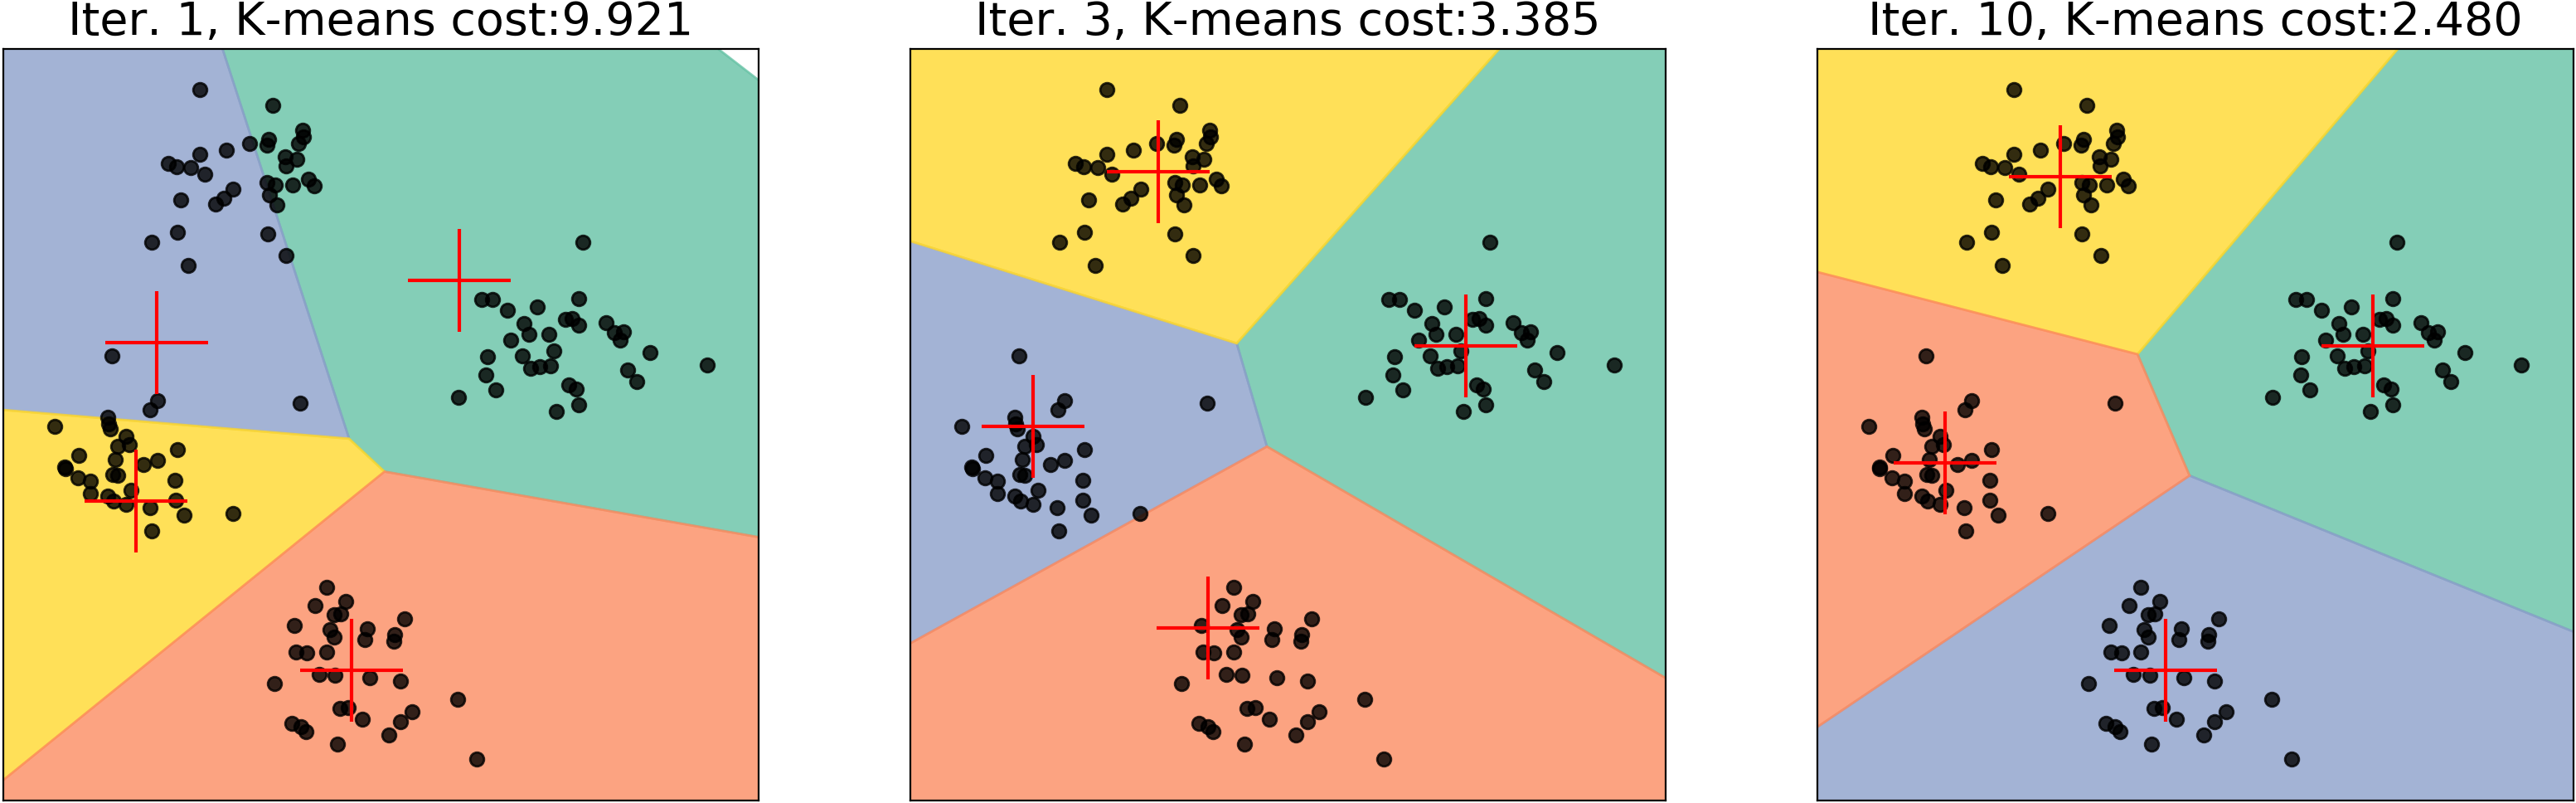
\includegraphics[scale=0.35]{TeX_files/voronoi_kmeans.png}
 \caption{Llyod's algorithm with random initialization centers and final Voronoi partitions at different steps: with 1 iteration (left), 3  (middle) and 10 (right) iterations (the algorithm converged). $K$-means costs are given on top.}
 \label{voronoi_graph}
 \end{figure}
\begin{figure}[h]
\begin{center}
\mybox{
\begin{minipage}{0.85\linewidth}
\begin{algorithmic}%[1]\tt
\small
\STATE {\bfseries Input:} N points $\bx_1,\ldots,\bx_n\in\RR^p$ and the number of clusters $K$.
\STATE {\bfseries Output:} Cluster centers $\hat\bc_1,\dots,\hat\bc_K$ and clusters assignments.
\STATE {\bfseries Init:} Set $\mathcal{L}_{\textnormal{old}}=\infty.$ and chose $K$ seed points $\bc_1,\dots,\bc_K$. Compute the $K$-means cost $\mathcal{L}_{\textnormal{curr}}$ given in \cref{kmeans_min_problem} with these points as centers.
\WHILE{$\mathcal{L}_{\textnormal{curr}}  < \mathcal{L}_{\textnormal{old}}$} 
\STATE{\tt 1: }Compute the Voronoi partitioning of the data with $\bc_1,\dots,\bc_K$ as centers. Get $K$ clusters, $C_1,\dots,C_K$.
\STATE{\tt 2: }On each clusters, compute the sample means $\hat\bc_1,\dots,\hat\bc_K$:
\begin{equation}
  \hat\bc_i = \frac{1}{|C_i|}\sum_{x_j\in C_i} x_j
\end{equation}
\STATE{\tt 3: }Set $\mathcal{L}_{\textnormal{old}} = \mathcal{L}_{\textnormal{curr}}$ and compute the new $K$-means cost $\mathcal{L}_{\textnormal{curr}}$ with $\hat\bc_1,\dots,\hat\bc_K$ as centers.
\ENDWHILE
\end{algorithmic}
\end{minipage}
}
   \caption{$K$-means Lloyd's algorithm}
   \label{algo:lloyd_algo}
\end{center}
\vspace{-15pt}
\end{figure}
 Note that Lloyd's algorithm has several drawbacks: 
\begin{enumerate}
\item It is a hard-assignment method since it assigns points to clusters and does not reflect a level of uncertainty on the assignments such as a probability of belonging to a cluster.
 \item The number of clusters has to be given, we will see some techniques to select the number of clusters in \cref{estim_nb_clusters_sect}.
 \item The worst-case time complexity $T(n)$ is superpolynomial, $T(n)=2^{\Omega(\sqrt{n})}$ iterations \citep{kmeans_slow_arthur_2016} (not bounded above by any polynomial). Fortunately, in practice it is observed that Lloyd's algorithm converges quickly to a local minimum.
 \item If the initial centers are chosen randomly, the resulting $K$-means cost can be made arbitrarily bad compared to the optimal clustering (see section 5.2 of \citep{hennig2015handbook}). $K$-means$++$ \citep{Arthur:2007:KAC:1283383.1283494} address this problem by choosing carefully the initializations centers in Lloyd's algorithm, see \Cref{algo:kmeans++_algo} for the procedure, and showed that $K$-means$++$ is a $\log K$ approximation algorithm for the $K$-means objective, see \Cref{kmeans++_theo}.
\begin{theorem}{\citep{Arthur:2007:KAC:1283383.1283494}}
\label{kmeans++_theo}
Let $S$ be the set of centers output by the algorithm $K$-means$++$ and $\mathcal{L}(S)$ be the $K$-means cost of the clustering obtained using $S$ as the centers. Then $\EE[\mathcal{L(S)}]\leq O(\log(K))\mathcal{L}^*$, where $\mathcal{L}^*$ is the cost of the optimal $K$-means solution. 
\end{theorem}
\item $K$-means can not distinguish noise or select relevant features. This last point is particularly important in the case of high dimensional data, since it is generally accepted that the most relevant clusters lies in subspaces of much smaller dimension, we will discuss this phenomenon in \cref{curse_dim_section}. An idea would be to adapt Lloyd's method to the weighted $p^{th}$-root of the Minkowski metric
\begin{equation}
  d_{\bw}(\bx,\by) = \sum_{l=1}^p w_l|\bx_l - \by_l|^p,
\end{equation}
with $\bw$ a weight vector updated at each iterations. A first method of weighted $K$-means has been introduced in \citep{makarenkov2001optimal} and further developed in \citep{Huang_mink_kmeans} ($WK$-Means) for the Euclidean norm. An extension to the Minkowski metric is proposed in \citep{CordeirodeAmorim:2012:MMF:2051369.2051484} ($MWK$-Means) that outperforms $K$-means and $WK$-Means. Note that the use of a different metric has a profound impact on the implementation and running costs since the computation of Minkowski centers is not straightforward.
\end{enumerate}
\begin{figure}[h]
\begin{center}
\mybox{
\begin{minipage}{0.85\linewidth}
\begin{algorithmic}%[1]\tt
\small
\STATE {\bfseries Input:} N points $\bx_1,\ldots,\bx_n\in\RR^p$ and the number of clusters $K$.
\STATE {\bfseries Init:} Chose one center $\bc_1$ uniformly at random among the data points and add it to the set $\mathcal{S}$.
\FOR{$j=2$ to $K$ } 
\STATE{\tt 1:} Chose a point $\bx$ with probability proportional to $\min_{\bc \in \mathcal{S}} d(\bx,\bc)^2$  and add it to $\mathcal{S}$.
\ENDFOR
\STATE {\tt 2:} Proceed with $K$-means algorithm and the set $\mathcal{S}$ as initialization clusters. 
\end{algorithmic}
\end{minipage}
}
   \caption{$K$-means$++$ algorithm}
   \label{algo:kmeans++_algo}
\end{center}
\vspace{-15pt}
\end{figure}
The research on $K$-means is dense and several variants of this method has been developed. For instance $K$-medoids \citep{KaufmanR90} uses points of the data as centers, Mini-batch $K$-means\citep{Sculley:2010:WKC:1772690.1772862} takes mini-batches of data to reduce significantly computational times without penalizing too much the $K$-means cost or clustering algorithms that enjoy strong theoretical guarantees on non-worst case scenarios using notion of stability\citep{Ostrovsky2006}. The reader can refer to \citep{hennig2015handbook} for further details on this topic.

\subsection{Agglomerative Hierarchical Methods}
The idea of Hierarchical clustering is to form a hierarchy of clusters (i.e. nested clusters) which might be interesting to see how clusters are related to each other (something we cannot see with $K$-means). This method of clustering is very popular due to its simplicity and the resulting structure and organization. There exists two types: agglomerative and divisive. The first type consists to start from $N$ sets, each containing one element of the dataset and merge sets iteratively into larger groups according to an agglomeration rule and a similarity, i.e. building a hierarchy, until finding only one cluster that contains the whole data. The similarity can be a Minkowski distance, the cosine similarity or other distance such as Hamming, Hellinger or Mahalanobis.  The divisive procedure is the opposite of the agglomerative, starting from the whole dataset and splitting iteratively until obtaining $N$ sets. Divisive methods are generally very expensive, with a complexity of $O(2^n)$ , and are therefore not used in practice.

Let us consider the agglomerative procedure and a metric $d$, a simple implementation is to build the dissimilarity matrix $S=(d_{ij}=d(i,j))_{i,j\in [N]^2}$ (which is symmetric) and consider the couple $(i,j)$ such that $d_{ij}$ is the smallest dissimilarity in $S$. We create a new object $i \cup j$, add it to the matrix $S$ with the rule $d_{i\cup j, k}=\min\{d_{ik},d_{jk}\}$ and remove the rows and columns of sets $i$ and $j$ in $S$. The iteration of this procedure leads to one final cluster containing all points in the dataset. This method is called Single linkage clustering \citep{Graham:1985:HMS:1435654.1436662} and is detailed in \Cref{algo:single_linkage_hier_algo}. This procedure has a complexity of $O(n^2)$\citep{hierarchicalMurtagh}. The hierarchy can be visualized via a binary tree called `dendrogram' in \Cref{dendrogram_graph}. This method has a severe drawback called `chaining phenomenon' where clusters can be merged due to close points even if it contains other points very distant. A alternative method called `Complete linkage clustering' solves this problem by taking the maximum instead of the minimum in step 1 of \Cref{algo:single_linkage_hier_algo}. 
 \begin{figure}[h]
 \center
 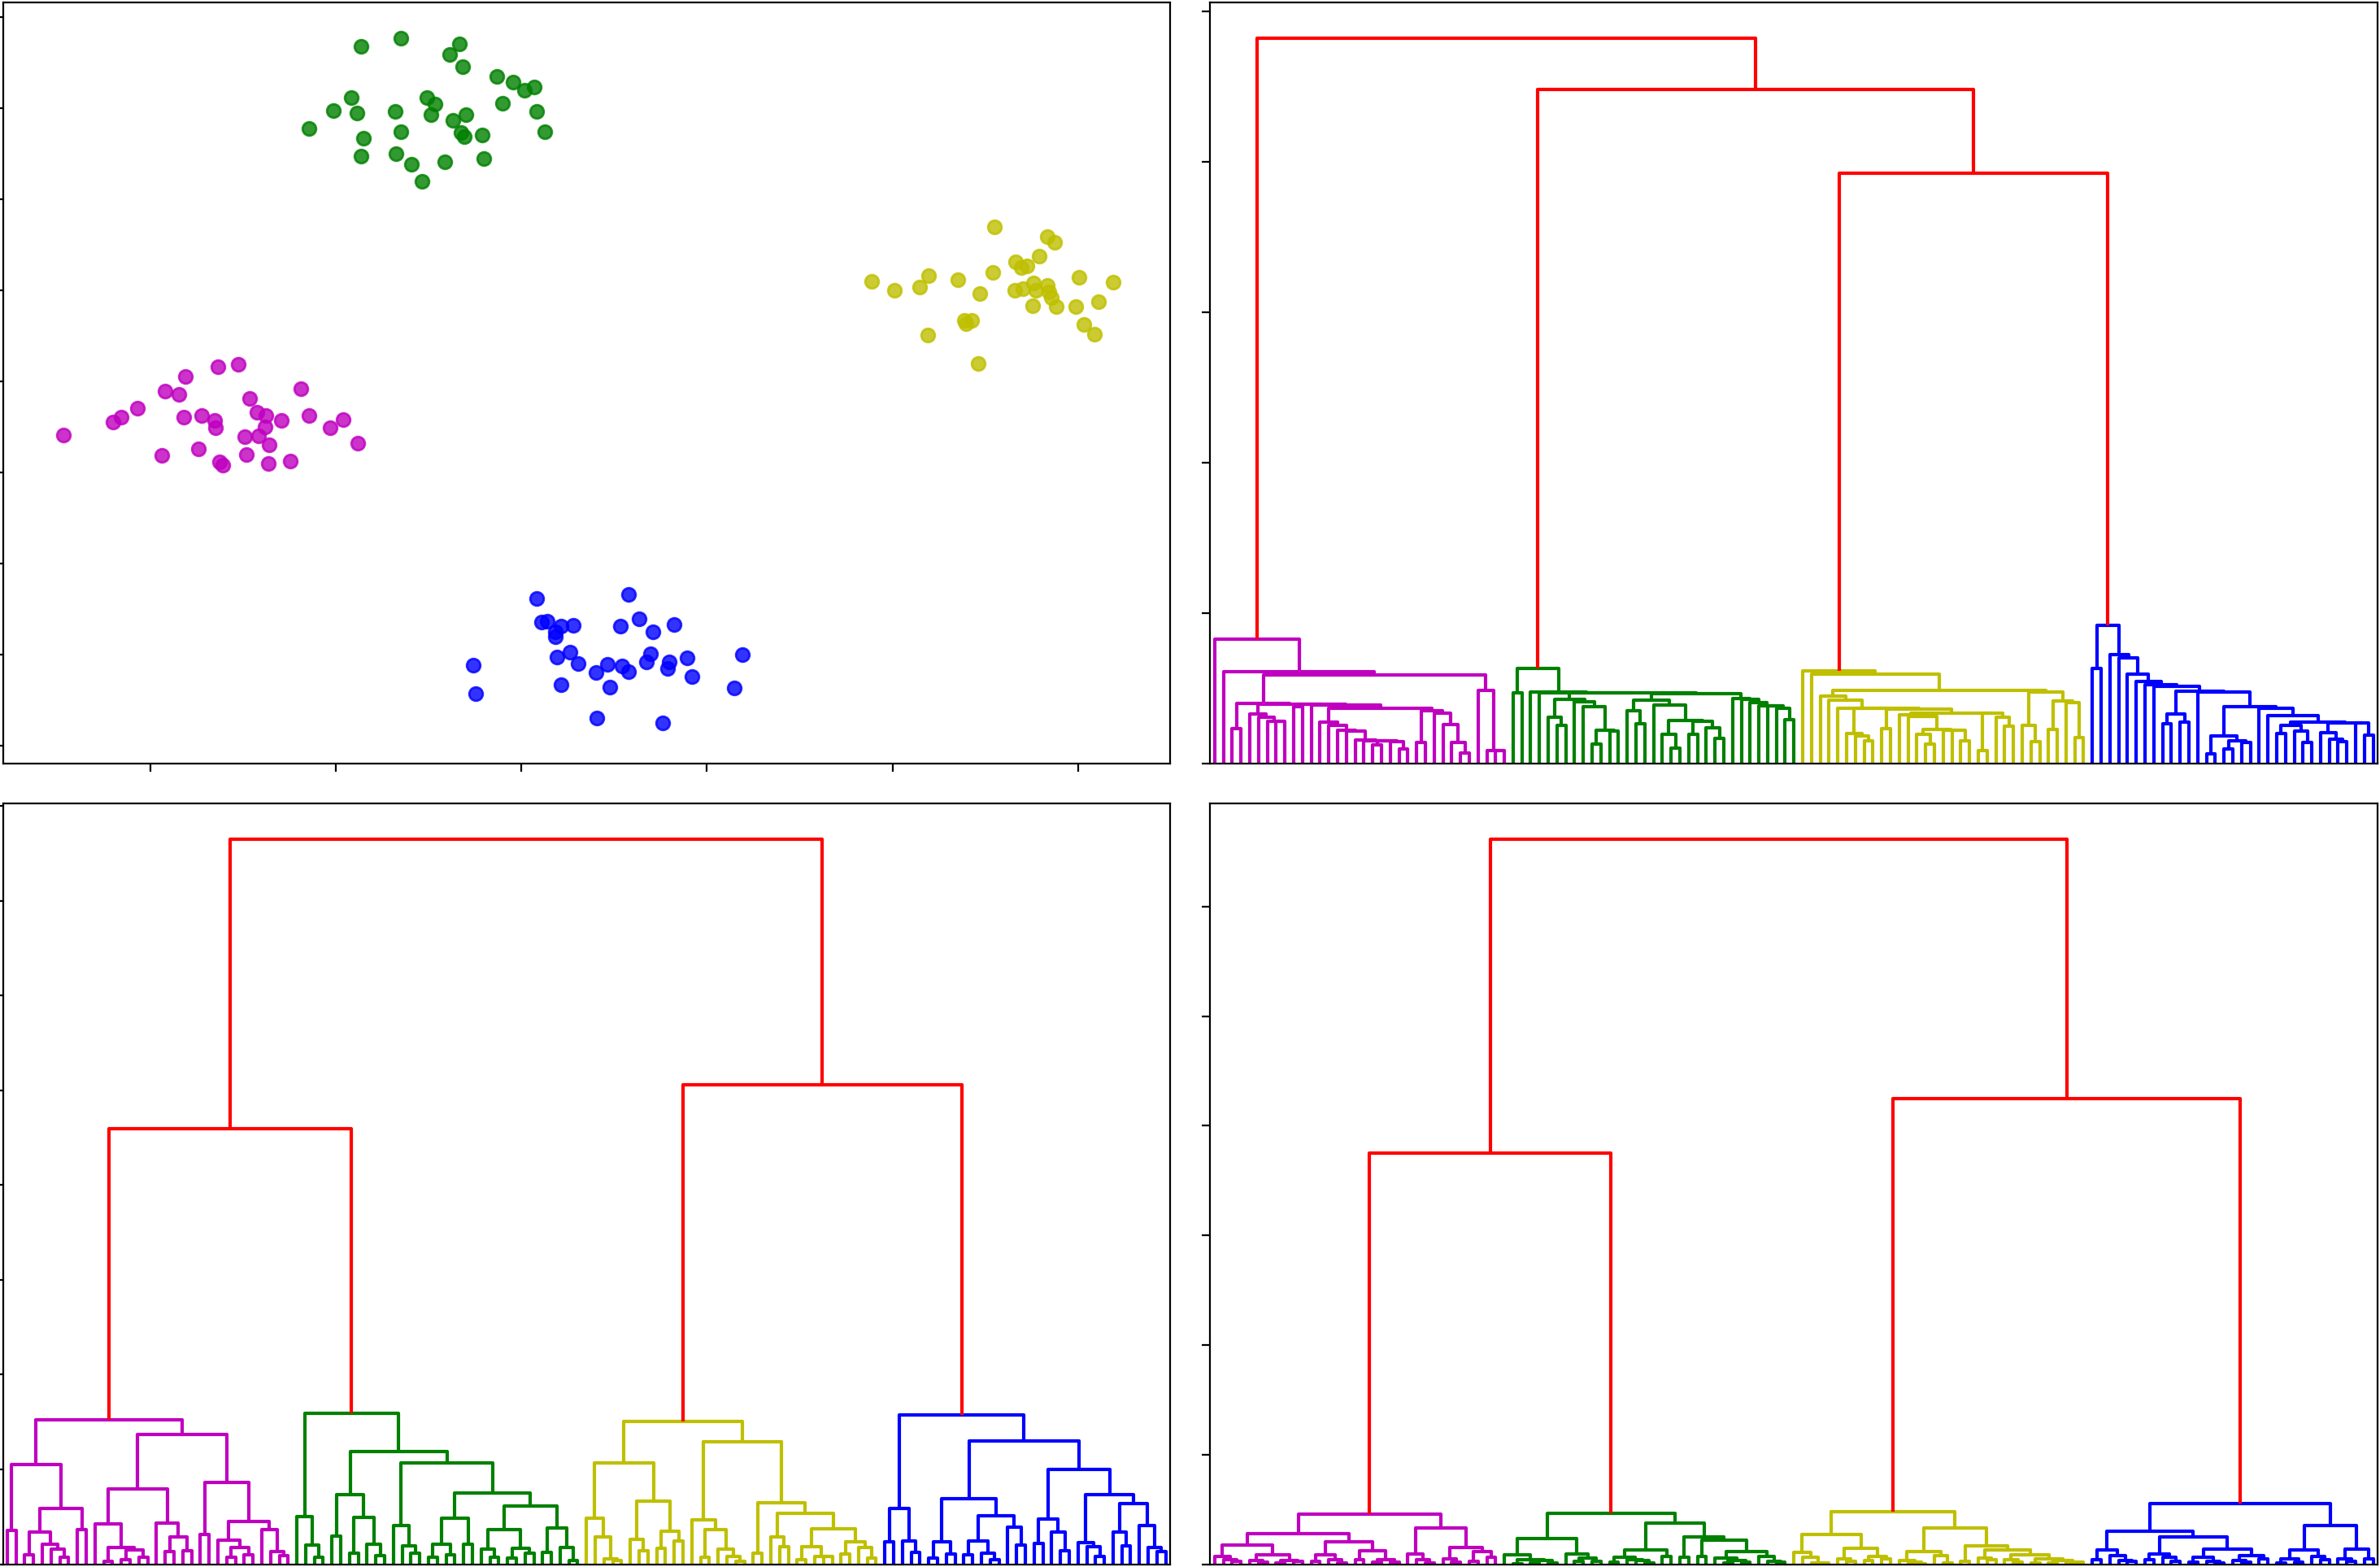
\includegraphics[scale=0.35]{TeX_files/dendrogram.png}
 \caption{The dataset with 4 clusters (top-left) used with the Agglomerative hierarchical clustering and its corresponding dendrogram, single-link (top-right), complete-link (bottom-left) and Ward's method (bottom-right). A simple way for finding clusters would be to cut the dendrogram with a horizontal line from bottom to top until finding the number of clusters desired. Note the difficulty to select the 4 original clusters.}
 \label{dendrogram_graph}
 \end{figure}
Lance and Williams developed an updating formula \citep{lance_williams_67} for the dissimilarities that generalize several methods of agglomerative methods. 
\begin{equation}
  d(i \cup j,k) = \alpha_id(i,k)+\alpha_jd(j,k)+\beta d(i, j) +\gamma |d(i,k)-d(j,k)|.
\end{equation}
For instance, the single-linkage method is recovered by setting $\alpha_i =\alpha_j = 1/2$, $\beta =0$ and $\gamma =-1/2$ and the complete-linkage method with $\alpha_i =\alpha_j = 1/2$, $\beta =0$ and $\gamma =1/2$. The reader can find parameters for other methods in Table 6.1 of \citep{hennig2015handbook}.
Another popular method worth mentioning for its use of cluster centers is the Ward's method\citep{ward63} also called Ward's minimum variance method which consists to optimize an objective function such as the sum of squares. Consider the merging cost of combining clusters $A$ and $B$:
\begin{align*}
  \Delta(A,B) &= \sum_{i\in A\cup B} \|\bx_i - \bc_{A \cup B} \|^2-\sum_{i\in A} \|\bx_i - \bc_{A} \|^2-\sum_{i\in B} \|\bx_i - \bc_{B} \|^2\\
  &= \frac{n_An_B}{n_A+ n_B}\|\bc_A - \bc_B \|^2,
\end{align*}
where $\bc_i$ is the center of cluster $i$.  This quantity is positive, hence the within-group variance increases when merging two clusters. Ward's method seek to minimize this growth. Note that Ward's method can be expressed in the Lance-Williams framework for evaluating $d(A \cup B, K)$ with $\alpha_i=(n_i+n_K)/(n_A+n_B+n_K)$, $\beta=-n_K/(n_A+n_B+n_K)$ and $\gamma=0$. More efficient algorithms relies on `Nearest Neighbor Chains'. Density based clustering

\begin{figure}[h]
\begin{center}
\mybox{
\begin{minipage}{0.85\linewidth}
\begin{algorithmic}%[1]\tt
\small
\STATE {\bfseries Input:} A dissimilarity matrix $S$.
\WHILE{at least 2 objects remain in S} 
\STATE{\tt 1:} Determine the smallest dissimilarity $d_{ij}$ in $S$.
\STATE{\tt 2:} Let $m$ be the size of $S$, compute the dissimilarities for the new cluster $i\cup j$:
\begin{equation}
  d_{i\cup j, k} = \min\{d_{ik},d_{jk}\},\quad k\in [m], m\neq i,j.
\end{equation}
\STATE{\tt 3:} Add the dissimilarities of $i\cup j$ in $S$ and remove those of clusters $i$ and $j$.
\ENDWHILE
\end{algorithmic}
\end{minipage}
}
   \caption{Simple single linkage hierarchical clustering}
   \label{algo:single_linkage_hier_algo}
\end{center}
\vspace{-15pt}
\end{figure}


\subsection{Spectral clustering}

\subsection{Finding the number of clusters}

\section{The Gaussian mixture model}

The Gaussian mixture model is an important framework for clustering problems. It assumes that the observations are drawn from a
mixture distribution the components of which are Gaussian  with parameters $(\bmu_k,\bSigma_k)$:
\begin{equation}
\varphi_{\bmu_k,\bSigma_k}(x)=\frac{1}{(2\pi)^{p/2}|\bSigma_k|^{1/2}} \exp\Big(-\frac{1}{2}(\bx-\bmu_k)^\top\bSigma_k^{-1}(\bx-\bmu_k)\Big)
\end{equation}

Let $\btheta$ be the list containing all the unknown parameters of a Gaussian mixture model: the family of means $\bmu = (\bmu_1,\ldots,\bmu_K)
\in (\RR^p)^K$, the family of covariance matrices $\bSigma = (\bSigma_1,\ldots,\bSigma_k)\in(\mathcal S_{++}^p)^K$ and the vector of cluster probabilities  $\bpi=(\pi_1,\ldots,\pi_k)\in [0,1]^K$ such that $\b1_p^\top\bpi=1$.
The density of one observation $\bX_1$ is then given by:
\begin{equation}\label{mixture}
p_{\btheta}(\bx)=\sum_{k=1}^K\pi_k\varphi_{\bmu_k,\bSigma_k}(\bx),\qquad \forall \bx\in\RR^p,
\end{equation}
where $\btheta=(\bmu,\bSigma,\bpi)$.


This model can be interpreted from a latent variable perspective. Let $Z$ be a discrete random variable
taking its values in the set $[K]$ and such that $\Pb(Z=k) = \pi_k$ for every $k\in[K]$. The random variable $Z$
indicates the cluster from which the observation $\bX$ is drawn.  Considering that all the conditional distributions
$\bX|Z=k$ are Gaussian, we get the following formula for the marginal density of $X$:
\begin{equation}
p_{\btheta}(\bx)=\sum_{k=1}^K \Pb(Z=k)p_{\theta}(\bx|Z=k) = \sum_{k=1}^K\pi_k\varphi_{\bmu_k,\bSigma_k}(\bx),\qquad \forall \bx\in\RR^p.
\end{equation}
In the clustering problem, the goal is to assign $X$ to a cluster or, equivalently, to predict the cluster $Z$ of the vector $\bX$.
A prediction function in such a context is $g:\RR^p\to[K]$ such that $g(\bX)$ is as close as possible to $Z$. If we measure the
risk of a prediction function $g$ in terms of misclassification error rate $R_\btheta(g) = \Pb_\btheta(g(\bX)\not=Z)$, then it is
well known that the optimal (Bayes) predictor $g^*_\btheta \in \arg\min_g R_\btheta(g)$ is provided by the rule
$$
g^*_\btheta(\bx) = \arg\max_{k\in [K]} \tau_k(\bx,\btheta),
$$
where $\tau_k(\bx,\btheta)=p_{\btheta}(Z=k|\bX=\bx)$ stands for the conditional probability of the latent variable $Z$ given $\bX$.
In the Gaussian mixture model, Bayes's rule implies that
\begin{equation}
\label{tau_bayes}
\tau_k(\bx,\btheta)=\frac{p_{\btheta}(\bx|Z=k)\Pb(Z=k)}{p_{\btheta}(\bx)}
=\frac{\pi_k\varphi_{\bmu_k,\bSigma_k}(\bx)}{\sum_{k'=1}^K\pi_{k'}\varphi_{\bmu_{k'},\bSigma_{k'}}(\bx)}
\end{equation}


Since the true value of the parameter $\btheta$ is not available, formula (\ref{tau_bayes}) can not be
directly used for solving the problem of clustering. Instead, a natural strategy is to estimate $\btheta$
by some vector $\hat\btheta$, based on a sample $\bX_1,\ldots,\bX_n$ drawn from the density $p_\btheta$, and
then to define the clustering rule by
\begin{equation}
\label{gen_clust}
\hat g(\bx) = g^*_{\hat\btheta}(\bx)=\arg\max_{k\in [K]} \tau_k(\bx,\hat\btheta)=\arg\max_{k\in [K]}\
\hat\pi_k\varphi_{\hat\bmu_k,\hat\bSigma_k}(\bx).
\end{equation}
A common approach to estimating the parameter $\btheta$ is to rely on the likelihood maximization.

Let $\bX_1,\dots,\bX_n$ with $\bX_i\in \RR^p$ be a set of iid observations drawn from the density $p_{\btheta}$
given by (\ref{mixture}). The following graphical model depicts the scheme of the observations:
%%GRAPH of pgm
\begin{figure}[h]
\centering\small
\begin{tikzpicture}
\tikzstyle{main}=[circle, minimum size = 6mm, thick, draw =black!80, node distance = 10mm]

\tikzstyle{connect}=[-latex, thick]
\tikzstyle{box}=[rectangle, draw=black!100]
  \node[main, fill = black!50] (x) [label=below:{$\bX_i$}] { };
  \node[main] (z) [above=of x,label=above:{$Z_i$}] {};

  \path (z) edge [connect] (x);

  \node[rectangle, inner sep=7mm,draw=black!100, fit= (z) (x)] {};
\node[rectangle, below=of x, inner sep=-10mm, fit= (z) (x),label=below right:{$\!\mathcal N$}, xshift=4mm,yshift=-2mm] {};

\node[main,draw=none] (a) [right=of x] {$\{\bmu_k\}$};
\path (a) edge [connect] (x);
\node[main,draw=none] (b) [left=of x] {$\{\bSigma_k\}$};
\path (b) edge [connect] (x);
\node[main,draw=none] (c) [right=of z] {$\{\pi_k\}$};
\path (c) edge [connect] (z);
\end{tikzpicture}
\end{figure}

The log-likelihood of the Gaussian mixture model is
\begin{equation}\label{log-likelihood}
\ell_n(\btheta)=\sum_{i=1}^{n}\log{p_{\btheta}(\bx_i)}=
\sum_{i=1}^{n}\log\bigg\{{\sum_{k=1}^K\pi_k\varphi_{(\bmu_{k},\bSigma_{k})}(\bx_i)}\bigg\}.
\end{equation}
Because of the presence in this equation of the logarithm of a sum, the maximization of the log-likelihood is
a difficult nonlinear and nonconvex problem. In particular, this is not a exponential family distribution yielding simple expressions.
A commonly used approach for approximately maximizing (\ref{log-likelihood}) with respect to $\btheta$ is the Expectation-Maximization
(EM) Algorithm \citep{dempster77} that we recall below.

Summarizing the content of this section, we can describe the following  natural approach to solving the clustering problem under Gaussian
mixture modeling assumption:
\begin{figure}[h]
\begin{center}
\mybox{
\begin{minipage}{0.85\linewidth}
\begin{algorithmic}%[1]\tt
\small
\STATE {\bfseries Input:} data vectors $\bx_1,\ldots,\bx_n\in\RR^p$ and the number of clusters $K$
\STATE {\bfseries Output:} function  $\hat g : \RR^p\to [K]$
\STATE {\tt 1: Estimate $\btheta=(\bpi,\bmu,\bSigma)$ by maximizing the log-likelihood:}
\begin{align}\label{step:1}
\hat\btheta
    &\in\arg\max_{\btheta\in\bTheta}  \ell(\btheta|\bx_1,\dots,\bx_n)
    =\arg\max_{\bpi,\bmu,\bSigma}  \sum_{i=1}^{n}\log\bigg\{{\sum_{k=1}^K\pi_k\varphi_{\bmu_{k},\bSigma_{k}}(\bx_i)}\bigg\}.
\end{align}
\STATE {\tt 2: Output the clustering rule:}
\begin{equation}
\label{step:2}
\hat g(\cdot) = \arg\max_{k\in [K]} \hat\pi_k\varphi_{\hat\bmu_k,\hat\bSigma_k}(\cdot).
\end{equation}
\end{algorithmic}
\end{minipage}
}
   \caption{Clustering under Gaussian mixture modeling}
   \label{algo:general}
\end{center}
\vspace{-15pt}
\end{figure}


\subsection{EM Algorithm}

The goal of the EM algorithm is to approximate a solution of the problem \eqref{step:1}.
Since this optimization problem contains a nonconvex cost function, it is impossible to
design a polynomial time algorithm that provably converges to the global maximum point. Instead,
the EM algorithm provides a sequence $\{\hat\btheta(t)\}_{t\in\NN}$ of parameter values such that
the cost function (\textit{i.e.}, the log-likelihood) evaluated at these values forms an
increasing sequence that converges to a local maximum.

The main idea underlying the EM algorithm is the following representation of the log-likelihood
of one observation derived from the log-sum inequality:
\begin{equation}\label{hint}
\log\bigg\{{\sum_{k=1}^K\pi_k\varphi_{\bmu_{k},\bSigma_{k}}(\bx_i)}\bigg\} =
\max_{\substack{\btau\in[0,1]^K \ \btau^\top \b1_K=1}} \sum_{k=1}^K \Big\{\tau_{k}\log\varphi_{\bmu_{k},\bSigma_{k}}(\bx_i)+\tau_{k} \log(\pi_k/\tau_{k})\Big\}.
\end{equation}
Let us denote by $\bTau = (\tau_{i,k})$ a $n\times K$ matrix with nonnegative entries such that $\bTau\b1_K = \b1_n$, that is each
row of $\bTau$ is a probability distribution on $[K]$. Combining \eqref{step:1} and \eqref{hint}, we get
\begin{align}\label{eq:3}
\hat\btheta
    &\in\argmax_{\btheta=(\bpi,\bmu,\bSigma)}\max_{\bTau}
    \sum_{i=1}^{N} \sum_{k=1}^K \Big\{\tau_{i,k}\log\varphi_{\bmu_{k},\bSigma_{k}}(\bx_i)+\tau_{i,k}
    \log(\pi_k/\tau_{i,k})\Big\}.
\end{align}
The great advantage of this new representation of the log-likelihood function is that the cost
function in \eqref{eq:3}, considered as a function of $\btheta$ and $\bTau$, is biconcave, \textit{i.e.},
it is concave with respect to $\btheta$ for every fixed $\bTau$ and concave with respect to $\bTau$ for
every fixed $\btheta$. In such a situation, one can apply the alternating maximization approach to sequentially
improve on an initial point. In the present context, an additional attractive feature of the cost function
in \eqref{eq:3} is that the two optimization problems involved in the alternating maximization procedure
admit explicit solutions.

\begin{figure}[ht]
\begin{center}
\mybox{
\begin{minipage}{0.85\linewidth}
\begin{algorithmic}%[1]\tt
%\SetLine%\SetAlgoLined
\small
\STATE {\bfseries Input:} data vectors $\bx_1,\ldots,\bx_n\in\RR^p$ and the number of clusters $K$
\STATE {\bfseries Output:} parameter estimate $\hat\btheta = \{\hat\bmu_k,\hat\bSigma_k,\pi_k\}_{k\in[K]}$
\STATE {\tt 1: Initialize $t=0$, $\btheta=\btheta^0$.}
\STATE {\tt 2: {\bf Repeat}}
\STATE \qquad {\tt 3: Update the parameter $\bTau$:}
\begin{align*}
\tau_{i,k}^{t}  &= \frac{\pi_k^{t}\varphi_{\bmu_k^{t},\bSigma_k^{t}}(\bx_i)}{\sum_{k'\in[K]}\pi^{t}_{k'}\varphi_{\bmu^{t}_{k'},\bSigma^{t}_{k'}}(\bx_i)}.
\end{align*}
\STATE \qquad{\tt 4: Update the parameter $\btheta$:}
\begin{align*}
\pi_k^{t+1}     &= \frac1n\sum_{i=1}^n \tau_{i,k}^t,\qquad
\bmu_k^{t+1}    = \frac1{n\pi_k^{t+1}}\sum_{i=1}^n \tau_{i,k}^t\bx_i,\\
\bSigma_k^{t+1} &= \frac1{n\pi_k^{t+1}}\sum_{i=1}^n \tau_{i,k}^t(\bx_i-\bmu_k^{t+1})(\bx_i-\bmu_k^{t+1})^\top.
\end{align*}
\STATE \qquad {\tt 5: increment $t$: $t=t+1$}.
\STATE {\tt 6: {\bf Until} stopping rule.}
\STATE {\tt 7: {\bf Return} $\btheta^{t}$}.
\end{algorithmic}
\end{minipage}}
   \caption{EM algorithm for Gaussian mixtures}
   \label{algo:EM}
\end{center}
\end{figure}


\begin{lem}
\label{lemma1}
Let us introduce the cost function
\begin{equation}
F(\btheta,\bTau) = \sum_{i=1}^{n} \sum_{k=1}^K \Big\{\tau_{i,k}\log\varphi_{\bmu_{k},\bSigma_{k}}(\bx_i)+\tau_{i,k}
    \log(\pi_k/\tau_{i,k})\Big\}.
\end{equation}
Then, the following two optimization problems
\begin{align}
\hat\btheta(\bTau)&\in \arg\max_{\btheta} F(\btheta,\bTau),\qquad \hat\bTau(\btheta)\in \arg\max_{\bTau} F(\btheta,\bTau)
\end{align}
has explicit solutions given by
\begin{align}
\label{em-sols}
\hat\pi_k     &= \frac1n\sum_{i=1}^n \tau_{i,k},\qquad\hat\bmu_k = \frac1{n\hat\pi_k}\sum_{i=1}^n \tau_{i,k}\bx_i ,\qquad \forall k\in[K],\\
\hat\bSigma_k &= \frac1{n\hat\pi_k}\sum_{i=1}^n \tau_{i,k}(\bx_i-\hat\bmu_k)(\bx_i-\hat\bmu_k)^\top,\qquad\forall k\in[K],\\
\hat\tau_{i,k}&= \frac{\pi_k\varphi_{\bmu_k,\bSigma_k}(\bx_i)}{\sum_{k'\in[K]}\pi_{k'}\varphi_{\bmu_{k'},\bSigma_{k'}}(\bx_i)},\qquad\forall k\in[K],\ \forall i\in[n] \label{tau_ik_em}.
\end{align}
\end{lem}

Based on this result, the EM algorithm is defined as in Figure~\ref{algo:EM}.
The algorithm operates iteratively and needs a criterion to determine when
the iterations should be stopped. There is no clear consensus on this point in the
statistical literature, but it is a commonly used  practice to stop when one of the
following conditions is fulfilled:
\begin{description}
\item[i)]  The number of iterations $t$ exceeds a pre-specified level $t_{\max}$.
\item[ii)] The increase of the log-likelihood over past $t_0$ iterations is not
significantly different from zero: $\ell_n(\btheta^{t})-\ell_n(\btheta^{t-t_0})\le \varepsilon$
for some pre-specified values $t_0\in\NN$ and $\varepsilon>0$.
\end{description}
EM is conceptually easy and each iteration increases the log-likelihood:
$$
\ell_n(\btheta^{t+1})\ge \ell_n(\btheta^{t}),\qquad \forall t\in\NN.
$$
The complexity at each step of the EM algorithm is $O(Knp^2)$ and
it usually requires many iterations to converge. In a high-dimensional setting
when $p$ is large, the quadratic dependence on $p$ may result in prohibitively
large running times. However, the computation of the elements of the covariance
matrices $\bSigma^t_k$ and the mean vectors $\bmu^t_k$ can be parallelized which
may lead to considerable savings in the running time.

\subsection{$K$-means from the EM angle}

In this section, we will see that the $K$-means problem is closely related to the EM algorithm. We rewrite the minimization problem of $K$-means defined in \cref{kmeans_min_problem} as following
\begin{equation}
  \min_{\bc_1,\dots,\bc_K}\min_{\bR \in \{0,1\}^{N\times K}}\sum_{i=1}^N\sum_{k=1}^K r_{ik}\|\bx_i - \bc_k \|^2,
\end{equation}
where the matrix $\bR$ follows the $1$-of-$K$ coding scheme, i.e. if a point $\bx_i$ is assigned to the cluster $m$, then $r_{im}=1$ and $r_{il}=0, \forall l\in [K] \neq m$. One can see the underlying iterative procedure, the first one consists to minimize the objective function with respect to $\bc_1,\dots,\bc_K$ with $\bR$ fixed (Maximization step) and the second one consists to minimize the objective function with respect to $\bR$ with $\bc_1,\dots,\bc_K$ fixed (Expectation step). Consider the \textbf{E}-step, the objective function is linear with respect to $\bR$.  It consists for a data point $\bx_i$, to find the cluster $k$ such that $k = \argmin_{j\in[K]}\|\bx_i-\bc_j\|^2$. For the \textbf{M}-step, setting the gradient with respect to $\bc_k$ to 0 gives us
\begin{equation}
  2\sum_{i=1}^N r_{ik} (\bx_i-\bc_k) = 0,
\end{equation}
which leads to
\begin{equation}
  \bc_k = \frac{\sum_{i=1}^N r_{ik}\bx_i}{\sum_{i=1}^N r_{ik}}.
\end{equation}
Since $\sum_{i=1}^Nr_{ik}$ is the size of the cluster $k$, we recovered the Lloyd's algorithm.

\section{The curse of dimensionality}
\label{curse_dim_section}
\todos{reecrire cette partie en commencant par le pb de la HD en stats en general, se baser sur les points de Giraud, puis une deuxieme sous section avec le cas du clustering et les pistes de resolution connues, ex: penalization, subspace clustering...}
\todos{Ajouter un tableau des differents types de modeles et le nombre de parametres}

The expression "Curse of dimensionality" introduced by R.Bellman \todos{citer} referes to the problems linked with high dimension. One can see that evaluating a function on the segment $(0,1)$ with a step size of $0.1$ is straightforward. However, evaluating the function in a grid of dimension 10 requires $10^{10}$ computations which can be intractable even today within a reasonable time. This is an important issue in the clustering context. In the Gaussian mixture model of $K$ components in dimension $p$, the number of parameters to estimate is:
\begin{equation}
   \nu = \underbrace{(K-1)}_\text{Weights}+ \underbrace{Kp}_\text{Means} + \underbrace{Kp(p-1)^2}_\text{Covariances Matrices}
 \end{equation}
 Moreover, the evaluation of $\hat\tau_{i,k}$ in \cref{tau_ik_em} needs to evaluate the inverse of the covariance matrix $\hat\bSigma_k$ which is called the precision matrix. If $n<<\nu$ the matrices $\hat\bSigma_k\, k=1,\dots,K$ are ill conditioned and the precision matrices are prone to large numerical errors or more often singular and the problem can not be solved. In \cref{chapgraphlasso}, we tackle this challenge by studying some nice structural properties of precision matrices.
However,  an interesting phenomenon occurs in high dimension, Scoot and Thomson \todos{cite} showed that high-dimensional spaces are mostly empty, Huber \todos{cite}\todos{attention de pas copier Bouveyron\cite{bouveyron:hal-00750909}} showed that the realizations of a $p$-dimensional random vector with a uniform probability distribution on the unit hypershpere lies with high probability close to the boundary of this hypershere. Therefore, the data belong mostly in a $p-1$ dimensional subspace. Therefore, in the clustering problem, different clusters may live on different subspaces \todos{subspace clustering}
\subsection{Bibliographic notes}
The reader can find a more thorough study of high dimensional statistics in \cite{giraud2014introduction}.  The reader can refer to \citep{bouveyron:hal-00750909} to have an overview of the different Gaussian mixture models for clustering in high dimension.

\section{Some contributions}
In this section, we present some works carried out during this thesis which have unfortunately not been able to be the subject of an in-depth study that can be published. The first part deals with the sparse hypothesis of the precision matrices within a high dimensional Gaussian mixture and adapts the single-component Graphical Lasso from \citep{glasso07} to the mixture setting. In the second part, we assume that the weight vector of the mixture is sparse in order to obtain an estimator of the number of components in the mixture that is generally unknown. 

\subsection{Graphical Lasso for Gaussian mixtures}\label{chapgraphlasso}

As we saw in the introduction chapter\todos{changer en section}, the number of free parameters in a full GMM with $K$ components in dimension $p$ are $(K-1)+Kp+Kp(p+1)/2$ which means that for $K=5$ and $p=100$ we have $125704$ parameters to estimate. In this high dimensional setting, the EM algorithm experiences severe performance degradation. In particular, the inversion of the covariance matrices are challenged. One way to tackle these problems is to use regularization. We will make the assumption on some structure on the inverse of the covariance matrix of a component called the precision or concentration matrix. The work presented in this chapter is inspired by \citep{glasso07}, \citep{banerjee}, \citep{yuanLin_graph} and \citep{meinshausen2006} in which they penalize the components of the precision matrix of a Gaussian graphical model. We generalize this work to the Gaussian mixture model.

\subsubsection{Introduction}
We consider $\bX=(\bX^{(1)},\dots,\bX^{(p)})$ a random vector admitting a $p$-dimensional normal distribution $\mathcal N(\bmu, \bSigma)$ with $\bSigma$ non-singular. One can construct an undirected graph $G=(V,E)$ with $p$ vertices corresponding to each coordinates and, $E=(e_{i,j})_{1\leq i < j \leq p}$, the edges between the vertices describing the conditional independence relationship among $\bX^{(1)},\dots,\bX^{(p)}$. 
If in this graph, $e_{i,j}$ is absent in $E$ if and only if $X^{(i)}$ and $X^{(j)}$ 
are independent conditionally to the other variables $\{X^{(l)}\}$ with $l\neq i,j$ (noted $X^{(i)} \ci X^{(j)}|X^{(l)}\, l\neq i,j$), then $G$ is called the Gaussian concentration graph model for the Gaussian random vector $\bX$. 
This property is particularly interesting in the study of the inverse of the covariance matrix. Let us denote $\bSigma^{-1}=\bOmega=(\omega_{i,j})$ the precision matrix. The components of this matrix verify $\omega_{i,j}=0$ if and only if $X^{(i)} \ci X^{(j)}$ conditionally to the other variables. We recall in the following lemma this well known result

\begin{lemma}[Conditional independence in Gaussian concentration graph model]
Consider $\bX=(\bX^{(1)},\dots,\bX^{(p)})$ a p-dimensional random vector with a multivariate normal distribution $\mathcal N(\bmu, \bSigma)$, note $\bSigma^{-1}=\bOmega=(\omega_{i,j})$, then $X^{(i)} \ci X^{(j)}|X^{(l)} \iff \omega_{i,j}=0$ with $l\neq i,j$ 
\end{lemma}
\begin{proof}
This result can be found in \citep{edwards2000introduction}, consider the density of $\bX$
\begin{equation}
  \varphi_{\bmu,\bSigma}(\bx)=\frac{1}{(2\pi)^{p/2}|\bSigma|^{1/2}} \exp\Big(-\frac{1}{2}(\bx-\bmu)^\top\bSigma^{-1}(\bx-\bmu)\Big),
\end{equation}
it can be rewritten as
\begin{equation}
  \varphi_{\bmu,\bSigma}(\bx) = \exp(\alpha + \beta^T\bx-\frac{1}{2}\bx^T\bOmega\bx),
\end{equation}
with $\beta=\bOmega\bmu$ and $\alpha=\frac{1}{2}\log(|\bOmega|)-\frac{1}{2}\bmu^T\bOmega\bmu-\frac{p}{2}\log(2\pi)$. Then, the previous equation can be rewritten as 
\begin{equation}
\label{exp_fam_cond_ind}
  \exp\big(\alpha + \sum_{j=1}^p\beta_j\bx^{(j)}-\frac{1}{2}\sum_{j=1}^p\sum_{(i=1)}^p\omega_{i,j}\bx^{(j)}\bx^{(i)}\big).
\end{equation}
Now, for $X,Y,Z$ three random variables, we have $X \ci Y|Z$ iff the joint density can be factorized into two factors $f_{X,Y,Z}(x,y,z)=h(x,z)g(y,z)$ with $h$ anf $g$ two functions. Then, at the light of  \cref{exp_fam_cond_ind}, we have $X^{(i)}\ci X^{(j)}|X^{(l)} \iff \omega_{i,j}=0$.
\end{proof}
The literature on this subject focused on a first hand on the estimation of the graph structure, \citep{dempster1972cov_select} developed a greedy forward or backward search method to estimate the set of non-zero components in the concentration matrix. The forward method relies on initializing an empty set and select iteratively an edge with an MLE fit for $\mathcal{O}(p^2)$ different parameters. The procedure stops according to a suitable selection criterion. The backward method performs in the same manner by starting with all edges and performing deletions. It is obvious that such methods are computationally intractable in high dimension. In \citep{meinshausen2006}, the authors studied a neighborhood selection procedure with lasso. The goal is to estimate the neighborhood $ne_{X^{(i)}}$ of a node $X^{(i)}$ which is the smallest subset of $G\setminus\{X^{(i)}\}$ such that $X^{(i)} \ci \big\{X^{(j)}: X^{(j)}\in G\setminus\{ne_{X^{(i)}}\}\big\} | X_{ne_{X^{(i)}}}$. The estimation of the neighborhood is cast as a regression problem with a lasso penalization. The authors showed that this procedure is consistent for sparse high dimensional graphs and computationally efficient. More precisely, let $\theta^{(i)} \in \RR ^p$ be the vector of coefficient of the optimal prediction,\todos{banerjee p488, consistency lies on choice of penalty}
\begin{equation}
  \theta^{(i)} = \argmin_{\theta:\theta_i=0}\EE\Big[ X^{(i)}-\sum_{k=1}^p\theta_k X^{(k)}\Big],
\end{equation}
then the components of $\theta^{(i)}$ are determined by the precision matrix, $\theta^{(i)}_j=-\omega_{i,j}/\omega_{i,i}$. Therefore, the set of neighbors of $X^{(i)}\in G$ is given by
\begin{equation}
  ne_{X^{(i)}}= \{X^{(j)}, j\in[p]: \omega_{i,j} \neq 0 \}.
\end{equation}
Now, let $\XX$ be the $n\times p$-dimensional matrix such that the column $\XX^{(i)}$ is the $n$ observations vector of $X^{(i)}$, given a regularization parameter $\lambda \geq 0$ carefully chosen, the Lasso estimate $\hat\theta^{i,\lambda}$ of $\theta^{(i)}$ is given by
\begin{equation}
  \hat\theta^{i,\lambda} = \argmin_{\theta:\theta_i=0}\Big(\frac{1}{n}\|\XX^{(i)}-\XX\theta \|_2^2 + \lambda\|\theta\|_1 \Big).
\end{equation}
The authors proved under several assumptions that 
\begin{equation}
  P(\hat{ne}_{X^{(i)}}^{\lambda}=ne_{X^{(i)}})\rightarrow 1 \quad \text{for}\, n\rightarrow \infty,
\end{equation}
and for some $\epsilon > 0$,
\begin{equation}
  P(\hat E^{\lambda}=E)=1-\mathcal{O}(\exp(-cn^{\epsilon}))\quad \text{for}\, n\rightarrow \infty.
\end{equation}
Therefore, this method recovers the conditional independence structure of sparse high-dimensional Gaussian concentration graph \todos{ajouter un mot sur la complexité} at exponential rates. However, this method performs model selection but does not estimate the parameters of the model. One  could estimate the parameters of a model which has been selected by this method. Such procedure often leads to instability of the estimator since small changes on the data would change the model selected \citep{yuanLin_graph}, \citep{breiman1996}. One major difficulty of a method that would perform both tasks is to ensure that the estimator of the precision matrix is positive definite. \citep{yuanLin_graph} proposed a penalized-likelihood method that performs model selection and parameter estimation simultaneously as well as ensuring the positive definiteness of the precision matrix. Their approach is similar to \citep{meinshausen2006} as they use the $\ell_1$ penalty but with the likelihood and the addition of a positive definite constraint. The log-likelihood for $\bOmega$ based on a  centered random sample $\bX_1,\dots,\bX_n$ of $\bX$ is
\begin{equation}
  \frac{n}{2}\log(|\bOmega|) - \frac{1}{2}\sum_{i=1}^n\bX_i^T\bOmega\bX_i
\end{equation}
and the constrained minimization problem over the set of positive definite matrices is
\begin{equation}
\label{prec_matrix_gauss_min_pb}
  \text{min}\Big\{-\log(|\bOmega|) + \frac{1}{n}\sum_{i=1}^n\bX_i^T\bOmega\bX_i\Big\} \quad \text{subject to}\quad \sum_{i\neq j} |\omega_{i,j}|\leq t,
\end{equation}
with $t\geq 0$ a tuning parameter. Note that $\hat\bmu=\bar\bX$. Consider the empirical covariance matrix $\bS=1/n\sum_{i=1}^n\bX_i^T\bX_i$, the \cref{prec_matrix_gauss_min_pb} can be rewritten as 
\begin{equation}
  \text{min}\Big\{-\log(|\bOmega|) + \text{tr}(\bS\bOmega)\Big\} \quad \text{subject to}\quad \sum_{i\neq j} |\omega_{i,j}|\leq t.
\end{equation}
Since the whole problem is convex, the Lagrangian form is given by
\begin{equation}
\label{yuan_lkhood_pb}
  \mathcal L (\lambda, \bOmega) = -\log(|\bOmega|) + \text{tr}(\bS\bOmega) + \lambda\sum_{i\neq j} |\omega_{i,j}|,
\end{equation}
with $\lambda$ the tuning parameter. A non-negative garrote-type estimator is provided in \citep{yuanLin_graph} but can be only applied when a good estimator of $\bOmega$ is available\todos{regarder de plus pres}. Therefore, we will continue our study of the Lasso-type estimator, the authors provided an asymptotic result
\begin{theorem}[Theorem 1 from \citep{yuanLin_graph}]
If $\sqrt{n}\lambda \rightarrow \lambda_0\geq0$  as $n\rightarrow\infty$, the lasso-type estimator is such that 
\begin{equation*}
  \sqrt{n}(\hat\bOmega-\bOmega)\rightarrow\argmin_{\bU=\bU^T}(V),
\end{equation*}
in distribution where
\begin{equation*}
  V(\bU)=\textnormal{tr}(\bU \bSigma \bU \bSigma)+\textnormal{tr}(\bU \bW)+\lambda_0\sum_{i\neq j}\big\{ u_{i,j}\textnormal{sign}(\omega_{i,j})I(\omega_{i,j}\neq 0)+|u_{i,j}|I(\omega_{i,j} =0) \big\}
\end{equation*}
in which $\bW$ is a random symmetric $p\times p$ matrix such that $\textnormal{vec}(\bW) \sim \mathcal N (0, \Lambda)$, and  $\Lambda$ is such that
\begin{equation*}
  \textnormal{cov}(w_{i,j},w_{i',j'}) = \textnormal{cov}(X^{(i)}X^{(j)},X^{(i')}X^{(j')}).
\end{equation*}
\end{theorem}\todos{mettre un commentaire sur ce resultat et aspect algorithmique}
Unfortunately, the computational complexity of interior point methods for maximizing \cref{yuan_lkhood_pb} is $\mathcal O (p^6)$ and at each steps, we have to compute and store a Hessian matrix of size $\mathcal O (p^2)$. These prohibitive complexities led the research on more specialized methods. \citep{banerjee} worked on the same approach, solving a maximum likelihood problem with an $\ell_1$ penalty and focusing on the computation complexity by proposing an iterative block coordinate descent algorithm. The problem to maximize is similar to \cref{yuan_lkhood_pb}
\begin{equation}
\label{max_lkhood_gauss_graph}
  \hat\bOmega = \argmax_{\bOmega \succ 0}\{\log(|\bOmega|)-\textnormal{tr}(\bS\bOmega)-\lambda\|\bOmega \|_1\}.
\end{equation}
Note that the $\ell_1$ norm of a matrix $\bOmega$ can be expressed as
\begin{equation}
  \|\bOmega \|_1 = \max_{\| \bU\|_{\infty}\leq 1}\textnormal{tr}(\bOmega\bU),
\end{equation}
injecting this in \cref{max_lkhood_gauss_graph} gives
\begin{equation}
  \max_{\bOmega \succ 0} \min_{\|\bU\|_{\infty}\leq \lambda} \big\{\log(|\bOmega|)-\textnormal{tr}(\bOmega(\bS+\bU))\big\}.
\end{equation}
After exchanging the min and the max, we solve the problem for $\bOmega$ by setting the gradient to $0$ which gives $(\bOmega^{-1})^T-(\bS+\bU)^T=0$ then $\bOmega = (\bS+\bU)^{-1}$. The dual problem is then
\begin{equation}
  \min_{\|\bU \|_{\infty}}\{-\log(|\bS+\bU|) -p\},
\end{equation}
or by setting $\bW = \bS+\bU$,
\begin{equation}
\label{banerjee_min_pb}
  \hat\bSigma = \hat{\bOmega^{-1}}= \argmax \log(|\bW|) \quad \textnormal{s.t}\quad \|\bW-\bS \|_{\infty} \leq \lambda.
\end{equation}
We observe the presence of a log-barrier adding the implicit constraint $(\bS+\bU) \succ 0$. Furthermore, the dual problem estimates the covariance matrix.\todos{pourquoi $\Sigma_{kk}=S_{kk}+\lambda ?$, p488}.\todos{citer les theoremes et choix du param}. To solve this maximization problem, the authors proposed a Block Coordinate Descent Algorithm described in \cref{fig:banerjee_block_algo}. For any symmetric matrix $\bA$, let $\bA_{\setminus k \setminus j}$ be the matrix produced by removing column $k$ and row $j$ to $\bA$. Let $\bA_j$ the $j^{th}$ column of $\bA$ with the element $\bA_{jj}$ removed.
\begin{figure}
\begin{center}
\mybox{
\begin{minipage}{1.1\linewidth}
\begin{algorithmic}[1]%\SetAlgoLined\tt\SetLine
\small
\STATE {\bfseries Input:} Matrix $\bS$, parameter $\lambda$ and threshold $\varepsilon$
\STATE {\bfseries Output:} Estimate of $\bW$
\STATE {{\bf Initialize} $\bW^{(0)} := \bS+\lambda I$}
\REPEAT
\FOR{$j=1,\dots,p$}
\STATE {(a) Let $\bW^{(j-1)}$ denote the current iterate. Solve the quadratic program}
\begin{equation*}
\label{banerjee_algo_min_pb}
  \hat \by := \argmin_{\by}\{\by^T(\bW_{\setminus j \setminus j}^{(j-1)})^{-1}\by:\|\by-\bS_j\|_{\infty}\leq \lambda\}.
\end{equation*}
\STATE {(b) Update the rule: $\bW^{(j)}$ is $\bW^{(j-1)}$ with column/row $\bW_j$ replaced by $\hat\by$.}
\ENDFOR
\STATE{Let $\hat\bW^{(0)}:=\bW^{(p)}$.}
\UNTIL{convergence occurs when
\begin{equation*}
  \textnormal{tr}\big((\hat\bW^{(0)})^{-1}\bS\big) -p +\lambda\big\|(\hat\bW^{(0)})^{-1} \big\|_1\leq \varepsilon.
\end{equation*}
}
\end{algorithmic}
\end{minipage}}
   \caption{Block Coordinate Descent Algorithm}
   \label{fig:banerjee_block_algo}

\end{center}
\end{figure}
They proved that the Block Coordinate Descent algorithm converges, achieving an $\varepsilon$-suboptimal solution to \cref{banerjee_min_pb} and each iterates produce a strictly positive definite matrix. For a fixed number of sweeps $K$, the complexity of this algorithm is $\mathcal O (Kp^4)$. They provide also another algorithm using Nesterov's first order method which has a $\mathcal O(p^{4.5}/\epsilon)$ complexity for $\varepsilon > 0$ the desired accuracy. It is interesting to note that the dual problem of \cref{banerjee_algo_min_pb} in \cref{fig:banerjee_block_algo} is 
\begin{equation}
  \min_{\bx} \bx^T\bW_{\setminus j \setminus j}^{(j-1)}\bx - \bS_j^T\bx + \lambda\|\bx\|_1,
\end{equation}
and strong duality holds, it can best casted as
\begin{equation}
\label{banerjee_dual_lasso}
  \min_{\bx} \|\bQ\bx - \bbb\|_2^2 + \lambda\|\bx\|_1,
\end{equation}
with $\bQ = (\bW_{\setminus j \setminus j}^{(j-1)})^{1/2}$ and $\bbb:=\frac{1}{2}\bQ^{-1}\bS_j$. Therefore, we recover the Lasso problem, more precisely, the algorithm can be interpreted as a sequence of iterative Lasso problems. This approach is similar to another paper that we would like to mention \citep{glasso07}. The authors proposed a faster algorithm based on the Block Coordinate Descent algorithm from \citep{banerjee} called Graphical Lasso. They estimate the matrix $\bW=\bOmega^{-1}$ by performing iterative permutations of the columns of this matrix to make the target column the last for a coupled Lasso problem. The matrices $\bW$ and $\bS$ will be presented as following 
\begin{equation}
\bW =  \begin{bmatrix}
    \bW_{11} & \bw_{12} \\
    \bw_{21} & w_{22}
  \end{bmatrix}, 
  \quad
 \bS =  \begin{bmatrix}
    \bS_{11} & \bs_{12} \\
    \bs_{21} & s_{22}
  \end{bmatrix}, 
\end{equation}
and the Graphical Lasso algorithm is described in \cref{fig:friedman_graph_lasso}. The Lasso problem can be solved via a coordinate descent, the reader can refer to \citep{glasso07} for the procedure. In this problem, the algorithm estimates $\hat\bSigma$ and returns also $\bB = (\bbb^{(1)},\dots,\bbb^{(p)})$, the matrix where each column is the solution of the Lasso problem in \cref{banerjee_dual_lasso} for each column of $\bW$. It is easy to recover $\bOmega$ since 
\begin{equation}
\bW =  \begin{bmatrix}
    \bW_{11} & \bw_{12} \\
    \bw_{21} & w_{22}
  \end{bmatrix}.
  \begin{bmatrix}
    \bOmega_{11} & \bomega_{12} \\
    \bomega_{21} & \omega_{22}
  \end{bmatrix}=
   \begin{bmatrix}
    I_{p-1} & 0 \\
    0 & 1
  \end{bmatrix},
\end{equation}
and
\begin{align*}
  \bomega_{12} &= -\bW_{11}^{-1}\bw_{12}\omega_{22}\\
  \omega_{22} &= 1/(w_{22}-\bw_{12}^T \bW_{11}^{-1}\bw_{12}).
\end{align*}
Therefore, for $j=1,\dots,p$, the permuted target components of $\bOmega$ are
\begin{align*}
  \bomega_{12} &= -\bbb^{(j)}\hat\omega_{22}\\
  \omega_{22} &= 1/(w_{22}-\bw_{12}^T \bbb^{(j)}).
\end{align*}
\begin{figure}
\begin{center}
\mybox{
\begin{minipage}{1.1\linewidth}
\begin{algorithmic}[1]%\SetAlgoLined\tt\SetLine
\small
\STATE {\bfseries Input:} Matrix $\bS$, parameter $\lambda$ and threshold $\varepsilon$
\STATE {\bfseries Output:} Estimate of $\bW$ and $\bB$ a matrix of parameters.
\STATE {{\bf Initialize} $\bW^{(0)} := \bS+\lambda I$ and $\bB=0_{p\times p}$. The diagonal of $\bW$ remained unchanged in what follows.}
\REPEAT
\FOR{$j=1,\dots,p$}
\STATE {(a) Let $\bW^{(j-1)}$ denote the current iterate. Solve the Lasso problem in \cref{banerjee_dual_lasso}
\begin{equation}
  \hat\bx^{(j-1)} = \argmin_{\bx} \frac{1}{2}\|(\bW_{11}^{(j-1)})^{1/2}\bx - \bbb\|_2^2 + \lambda\|\bx\|_1,
 \end{equation}
 with $\bbb:=(\bW_{11}^{(j-1)})^{-1/2}\bs_{12}$.}
\STATE {(b) Update: $\bW^{(j)}$ is $\bW^{(j-1)}$ with $\bw_{12}=\bW_{11}^{(j-1)}\hat\bx^{(j-1)}$. }
\STATE {(c) Save the parameter $\bx^{(j-1)}$ in the $j^{th}$ column of $\bB$.} 
\STATE{(d) Permute the columns and rows of $\bW^{(j-1)}$ such that the $j^{th}$ column is $\bw_{12}$, the next target.}
\ENDFOR
\STATE{Let $\hat\bW^{(0)}:=\bW^{(p)}$.}
\UNTIL{convergence occurs.}
\end{algorithmic}
\end{minipage}}
   \caption{Graphical Lasso}
   \label{fig:friedman_graph_lasso}

\end{center}
\end{figure}
In what follows, we will adapt these methods on a Gaussian mixture models, more precisely we will assume that each clusters present a sparse Gaussian concentration graph. We will rely on the Graphical Lasso for estimating the precision matrix and derive a EM algorithm.

\subsubsection{Graphical Lasso on Gaussian mixtures}

In this section, we present our contribution. We consider a Gaussian mixture model of $K$ components and our task is to estimate the parameters $\btheta=(\theta_1,\dots,\theta_K)$ with $\theta_k=(\pi_k, \bmu_k, \bOmega_k)$ where $\bOmega_k$ is the precision matrix regarding the $k^{th}$ component of the mixture. We denote $\varphi_{(\bmu_{k},\bOmega_{k})}$ the Gaussian density of mean $\bmu_k$ and precision matrix $\bOmega_k$. The penalized log-likelihood is

\begin{equation}
\label{pen-log-likelihood}
\ell_n^{pen}(\btheta)=\sum_{i=1}^{n}\log p_{\btheta}(\bx_i)-pen(\btheta)= \sum_{i=1}^{n}\log \bigg\{ \sum_{k=1}^K\pi_k\varphi_{(\bmu_{k},\bOmega_{k})}(\bx_i)\bigg\} -pen(\btheta).
\end{equation}
We suppose that each component of the mixture has a sparse Gaussian concentration graph. Therefore, in the scope of \citep{banerjee} and \citep{glasso07}, we consider an $\ell_1$ regularization $pen(\theta_k)=\sum_{k=1}^K\lambda_k||\bOmega_k||_{1,1}$ with $\lambda_k >0$. The penalization of the log-likelihood concerns only the precision matrices $\bOmega_k$. Regarding the other parameters $(\pi_k, \bmu_k)$, our algorithm is the same as EM and we can use the same iteration technique as in \cref{lemma1} to maximize the following cost function
\begin{equation}
\label{cost_fun_pen}
F^{pen}(\btheta,\bTau)  = \sum_{k=1}^K \bigg(\sum_{i=1}^{n} \Big\{\tau_{i,k}\log\varphi_{\bmu_{k},\bOmega_{k}}(\bx_i)+\tau_{i,k}
    \log(\pi_k/\tau_{i,k})\Big\}-\lambda_k||\bOmega_k||_{1,1}\bigg).
\end{equation}

The maximization of this function over $\btheta$ and $\bTau$ leads to the two following optimization problems\todos{ajouter les domaines}
\begin{align}
\label{optim-problems}
\hat\btheta(\bTau)&\in \arg\max_{\btheta} F^{pen}(\btheta,\bTau),\qquad \hat\bTau(\btheta)\in \arg\max_{\bTau} F^{pen}(\btheta,\bTau).
\end{align}
For a given $\hat\bTau$, estimates of $(\pi_1,\dots,\pi_K$ and $\bmu_1,\dots,\bmu_K)$ obtained by the first optimization problem in \cref{optim-problems} are the same as in the EM algorithm
\begin{align}
\label{em-sols}
\hat\pi_k     &= \frac1n\sum_{i=1}^n \hat\tau_{i,k},\quad\text{and}\quad\hat\bmu_k = \frac1{n\hat\pi_k}\sum_{i=1}^n \hat\tau_{i,k}\bx_i ,\qquad \forall k\in[K]
\end{align}
And for a given $\hat\btheta$, the estimate of $\bTau$ obtained by the second optimization problem is
\begin{equation}
\label{em-sols-tau}
\hat\tau_{i,k} = \frac{\hat\pi_k\varphi_{\hat\bmu_k,\hat\bOmega_k}(\bx_i)}{\sum_{k'\in[K]}\hat\pi_{k'}\varphi_{\hat\bmu_{k'},\hat\bOmega_{k'}}(\bx_i)}=p_{\btheta}(Z=k|\bX=\bx_i),\qquad\forall k\in[K],\ \forall i\in[n].
\end{equation}
However, due to the penality $\lambda_k||\bOmega_k||_{1,1}$, the estimation of $\bOmega_k$ is not straightforward.

We introduce the weighted empirical covariance matrix
\begin{equation}
\bSigma_{n,k} = \frac{1}{n}\frac{\sum_{i=1}^n\tau_{i,k}(\bx_i-\hat\bmu_k)(\bx_i-\hat\bmu_k)^\top}{\sum_{i=1}^n\tau_{i,k}}
\end{equation}
The Gaussian density in equation \eqref{cost_fun_pen} can be expanded as follows
\begin{align*}
\label{cost_fun_pen_2}
F^{pen}(\btheta,\bTau)  =& \sum_{k=1}^K \bigg( \sum_{i=1}^{n}\Big\{ \tau_{i,k} \Big(
-\frac{p}{2}\log(2\pi)+\frac{1}{2}\log|\bOmega_k|\\
&-\frac{1}{2}(\bx_i-\bmu_k)^T\bOmega_k(\bx_i-\bmu_k) \Big)+\tau_{i,k} \log(\pi_k/\tau_{i,k})\Big\} -\lambda_k||\bOmega_k||_{1,1}\bigg)\\
=& -\frac{np}{2}\log(2\pi)+\sum_{k=1}^K \bigg(\frac{n\pi_k}{2}\log|\bOmega_k|\\
&+\sum_{i=1}^{n}\Big\{ -\frac{\tau_{i,k}}{2}(\bx_i-\bmu_k)^T\bOmega_k(\bx_i-\bmu_k)+\tau_{i,k} \log(\pi_k/\tau_{i,k})\Big\} -\lambda_k||\bOmega_k||_{1,1}\bigg). 
\end{align*}

The opposite minimization problem regarding each $\bOmega_k$ is
\begin{equation}
\bOmega_k \in \argmin_{ \bOmega\succeq 0}\Big\{-\frac{n\pi_k}{2}\log|\bOmega|+\frac{1}{2}\sum_{i=1}^{n}\tau_{i,k}(\bx_i-\bmu_k)^T\bOmega(\bx_i-\bmu_k)+\lambda_k||\bOmega||_{1,1}\Big\}
\end{equation}
Using the well-known commutativity property of the trace operator and dividing by $n\pi_k$
\begin{equation}
\bOmega_k \in \argmin_{ \bOmega\succeq 0} \Big\{ -\frac{1}{2}\log|\bOmega| +\frac{1}{2} tr(\bSigma_{n,k}\bOmega)+\frac{\lambda_k}{n\pi_k}||\bOmega||_{1,1}\Big\}
\end{equation}

Our algorithm solves a graphical lasso problem within each cluster. We use a block coordinate ascent algorithm \citep{mazum_lasso} to solve this convex problem as in the graphical lasso implementation in R, see \url{http://statweb.stanford.edu/~tibs/glasso/} The alternating maximization procedure is summarized in the following algorithm
\begin{figure}
\begin{center}
\mybox{
\begin{minipage}{0.85\linewidth}
\begin{algorithmic}%\SetAlgoLined\tt\SetLine
\small
\STATE {\bfseries Input:} data vectors $\bx_1,\ldots,\bx_n\in\RR^p$ and the number of clusters $K$
\STATE {\bfseries Output:} parameter estimate $\hat\btheta = \{\hat\bmu_k,\hat\bOmega_k,\hat\pi_k\}_{k\in[K]}$
\STATE {\tt 1: Initialize $t=0$, $\btheta=\btheta^0$.}
\STATE {\tt 2: {\bf Repeat}}
\STATE {\tt 3: \qquad Update the parameter $\bTau$:}
\begin{align*}
\tau_{i,k}^{t}  &= \frac{\pi_k^{t}\varphi_{\bmu_k^{t},\bOmega_k^{t}}(\bx_i)}{\sum_{k'\in[K]}\pi^{t}_{k'}\varphi_{\bmu^{t}_{k'},\bOmega^{t}_{k'}}(\bx_i)}.
\end{align*}
\STATE {\tt 4: \qquad Update the parameter $\btheta$:}
\begin{align*}
\pi_k^{t+1}     &= \frac1n\sum_{i=1}^n \tau_{i,k}^t,\qquad \\
\bmu_k^{t+1}    &= \frac1{n\pi_k^{t+1}}\sum_{i=1}^n \tau_{i,k}^t\bx_i\\
\bSigma_{n,k}         &= \frac{1}{n^2\pi_k^{t+1}}\sum_{i=1}^n\tau_{i,k}^{t+1}(\bx_i-\hat\bmu_k^{t+1})(\bx_i-\hat\bmu_k^{t+1})^\top\\
\bOmega_k^{t+1} & \in \argmin_{ \bOmega\succeq 0} \Big\{ -\frac{1}{2}\log| \bOmega |+\frac{1}{2} tr(\bSigma_{N,k}\bOmega)+\frac{\lambda_k}{n\pi_k^{t+1}}||\bOmega||_{1,1}\Big\}
\end{align*}
\STATE {\tt 5: \qquad increment $t$: $t=t+1$}.
\STATE {\tt 6: {\bf Until} stopping rule.}
\STATE {\tt 7: {\bf Return} $\btheta^{t}$}.
\end{algorithmic}
\end{minipage}}
   \caption{Graphical lasso algorithm for Gaussian mixtures}
   \label{algo:PEM}
\end{center}
\end{figure}

%!TEX root = ../main.tex

\subsection{Estimating the number of clusters}
\label{estim_nb_clusters_sect}
In this chapter, we will focus on the open problem of estimating the number of clusters. Most of current clustering methods such that K-Means, Expectation-Maximisation with Gaussian mixture model or hierarchical clustering need a this parameter in input. Different methods are being used to perform a selection of the best model according to a criterion, unfortunately with a computational cost. In this work, we will try to tackle this challenge.

\subsubsection{Introduction and related work}
In previous models, we knew the number of components $K$ in the Gaussian mixture. In reality this parameter is unknown. 
Several methods exists to select the number of clusters

\subsubsection{Bayesian Information Criterion (BIC)}
A common method to select the number of clusters is to use the Bayesian Information Criterion given by:
\begin{equation}
  BIC(K) = -\log\ell_n(\hat\btheta^K)+K.\log(n)
\end{equation}
And select the model which minimizes the BIC. This can be done by running EM algorithm over a large number of models which is computationally expensive.

\subsubsection{Our First method}

The idea is to add a regularization term on the estimation of the $n\times K$ matrix $\bTau$, the estimate of the number of clusters K will be the number of non-empty columns of $\bTau$.\

We consider a maximum number of clusters $M$, we note the convex set $A=\{\tau \in \RR^M : \sum_{k=1}^M\tau_k=1, \tau_k\geq 0 \quad \forall k \in [M] \}$ and the "indicator" function $\chi_A(.)$ defined by:


  \begin{equation*}
    \chi_A(x) =
    \begin{cases}
      0 & \text{if } x \in A,\\
        \infty & \text{if } x = 0
    \end{cases}
\end{equation*}

We note $\bTau_{.,k}$ the $k^{th}$ column and $\bTau_{i,.}$ the $i^{th}$ line of $\bTau$. We will estimate $\bTau$ using the same equation \ref{cost_fun_pen}, \ref{optim-problems} with a regularization term:\\
\begin{align*}
F^{pen}(\btheta,\bTau)  =& \sum_{k=1}^K \bigg(\sum_{i=1}^{n} \Big\{\tau_{i,k}\log\varphi_{\bmu_{k},\bOmega_{k}}(\bx_i)+\tau_{i,k}
    \log(\pi_k/\tau_{i,k})\Big\}-\lambda_k||\bOmega_k||_{1,1}\bigg)\\ 
    &+ \sum_{k=1}^K ||\bTau_{.,k}||_{2} + \sum_{i=1}^{n} \chi_A(\bTau_{i,.})
\end{align*}
Removing the penalization on $\bOmega$:

\begin{align*}
F^{pen}(\btheta,\bTau)  =& \sum_{k=1}^K \bigg(\sum_{i=1}^{n} \Big\{\tau_{i,k}\log\varphi_{\bmu_{k},\bOmega_{k}}(\bx_i)+\tau_{i,k}
    \log(\pi_k/\tau_{i,k})\Big\}\\ 
    &+ \sum_{k=1}^K ||\bTau_{.,k}||_{2} + \sum_{i=1}^{n} \chi_A(\bTau_{i,.})
\end{align*}

 and the optimization problem:
\begin{equation}
\hat\bTau(\btheta)\in \arg\max_{\bTau} F^{pen}(\btheta,\bTau)
\end{equation}

Unfortunately, the regularization term prevents to derive explicit solution as in previous chapters. Furthermore, we cant separate the objective function since we optimize along columns and lines of $\bTau$. The objective function $F^{pen}(\btheta,\bTau)$ rewritten
$F^{pen}_{\btheta}(\bTau)$ can be split into two terms:

\begin{equation}
F^{pen}_{\btheta}(\bTau)={\large f}({\footnotesize
\bTau})+ {\large g}({\footnotesize
\bTau})
\end{equation}

with:

\begin{align*}
f(\bTau) =&   \sum_{k=1}^K \bigg(\sum_{i=1}^{n} \Big\{\tau_{i,k}\log\varphi_{\bmu_{k},\bOmega_{k}}(\bx_i)+\tau_{i,k} \log(\pi_k/\tau_{i,k})\Big\} + \sum_{k=1}^K ||\bTau_{.,k}||_{2}\\
g(\bTau) =& \sum_{i=1}^{n} \chi_A(\bTau_{i,.})
\end{align*}

$f$ is convex and differentiable on its domain, $g$ is also convex but not smooth. We will tackle this problem by using a proximal method:

\begin{align*}
  \bTau^{k+1} =& {\bf{prox}}_{\lambda g}(\bTau^k - \lambda \nabla f(\bTau^k))\
      =& P_A(\bTau^k - \lambda \nabla f(\bTau^k))\\
      =&\argmin_{ \bTau : \forall K, \bTau^k \in A}\big( || \bTau - (\bTau^k - \lambda \nabla f(\bTau^k) ) ||^2_2 \big)
\end{align*}

The gradient of f on $\bTau$ is given by:

\begin{align*}
\bigg[\nabla_{\bTau}f(\bTau)\bigg]_{i,j} =& \bigg[\frac{\partial f}{\partial \bTau_{ij}}(\bTau) \bigg]_{i,j}\\
=& \log(\varphi_{\bmu_j,\bOmega_j}(x_i))+\log(\frac{\pi_j}{\tau_{i,j}})+\frac{\tau_{i,j}}{||\bTau_{.,j}||_2}-1
\end{align*}

We will use FISTA to accelerate the convergence

\begin{figure}
\begin{center}
\mybox{
\begin{minipage}{0.85\linewidth}
\begin{algorithmic}%\SetAlgoLined\tt\SetLine
\small
\STATE {\bfseries Input:} 
\STATE {\bfseries Output:} parameter estimate $\bTau$
\STATE {\tt 1: Initialize $t_1=1$ and $\bxi^0$ with}
\begin{align*}
\xi_{i,k}^{0}  &= \frac{\pi_k^{0}\varphi_{\bmu_k^{0},\bOmega_k^{0}}(\bx_i)}{\sum_{k'\in[K]}\pi^{0}_{k'}\varphi_{\bmu^{0}_{k'},\bOmega^{0}_{k'}}(\bx_i)}
\end{align*}
\STATE {\tt 2: {\bf Repeat}}
\begin{align*}
\bTau^k =&\argmin_{ \bTau : \forall K, \bTau^k \in A}\big( || \bTau - (\bxi^k - \lambda \nabla f(\bxi^k) ) ||^2_2 \big)\\
t^{k+1} =& \frac{1+\sqrt{1+4*(t^k)^2}}{2}\\
\bxi^{k+1} =& \bTau^k + \bigg( \frac{t^k-1}{t^{k+1}}\bigg) \big( \bTau^k - \bTau^{k-1} \big)
\end{align*}
\end{algorithmic}
\end{minipage}}
   \caption{ $\bTau$ estimation with FISTA}
   \label{algo:PEM}
\end{center}
\end{figure}

We use the algorithm of last chapter with the new estimation procedure of $\bTau$ 

\begin{figure}
\begin{center}
\mybox{
\begin{minipage}{0.85\linewidth}
\begin{algorithmic}%\SetAlgoLined\tt\SetLine
\small
\STATE {\bfseries Input:} data vectors $\bx_1,\ldots,\bx_n\in\RR^p$ and the number of clusters $K$
\STATE {\bfseries Output:} parameter estimate $\hat\btheta = \{\hat\bmu_k,\hat\bOmega_k,\hat\pi_k\}_{k\in[K]}$
\STATE {\tt 1: Initialize $t=0$, $\btheta=\btheta^0$.}
\STATE {\tt 2: {\bf Repeat}}
\STATE {\tt 3: \qquad Update the parameter $\bTau$ with previous algorithm}
\STATE {\tt 4: \qquad Update the parameter $\btheta$:}
\begin{align*}
\pi_k^{t+1}     &= \frac1n\sum_{i=1}^n \tau_{i,k}^t,\qquad \\
\bmu_k^{t+1}    &= \frac1{n\pi_k^{t+1}}\sum_{i=1}^n \tau_{i,k}^t\bx_i\\
\bSigma_{n,k}         &= \frac{1}{n^2\pi_k^{t+1}}\sum_{i=1}^n\tau_{i,k}^{t+1}(\bx_i-\hat\bmu_k^{t+1})(\bx_i-\hat\bmu_k^{t+1})^\top\\
\bOmega_k^{t+1} & \in \argmin_{ \bOmega\succeq 0} \Big\{ -\frac{1}{2}\log| \bOmega |+\frac{1}{2} tr(\bSigma_{N,k}\bOmega)+\frac{\lambda_k}{n\pi_k^{t+1}}||\bOmega||_{1,1}\Big\}
\end{align*}
\STATE {\tt 5: \qquad increment $t$: $t=t+1$}.
\STATE {\tt 6: {\bf Until} stopping rule.}
\STATE {\tt 7: {\bf Return} $\btheta^{t}$}.
\end{algorithmic}
\end{minipage}}
   \caption{Graphical lasso algorithm for Gaussian mixtures with cluster number discovery}
   \label{algo:PEM}
\end{center}
\end{figure}


\subsection{Sparse Weights Vector Estimation}

 We fit a model with an arbitrarily large number of components $K$ and penalyze the weights vector $\bpi$. The penalized negative log-likelihood is:
\begin{equation}
  \ell_n(\btheta)=
-\frac{1}{n}\sum_{i=1}^{n}\log\bigg\{{\sum_{j=1}^K\pi_k\varphi_{(\bmu_{j},\bSigma_{j})}(\bx_i)}\bigg\}+\lambda\sum_{j=1}^{K-1}\pi_j^{1/\gamma}\quad \gamma\geq1
\end{equation}
Such that:
\begin{equation}
  \sum_{j}^{K-1}\pi_j \leq 1 \quad \text{and} \quad \pi_{K}=1-\sum_{j}^{K-1}\pi_j
\end{equation}
and $\sum_{j}^{K-1}\pi_j^{1/\gamma}$ is not convex, to rectify it let note $\alpha_j = \pi^{1/\gamma}$, then:
\begin{equation}
\hat\balpha\in\argmin_{\balpha\in \RR^{K-1}}\bigg\{
-\frac{1}{n}\sum_{i=1}^{n}\log\Big\{{\sum_{j=1}^K\alpha^\gamma_j\varphi_{(\bmu_{j},\bSigma_{j})}(\bx_i)}\Big\}+\lambda\sum_{j=1}^{K-1}\alpha_j \color{black} \bigg\}\quad \gamma\geq1,  
\end{equation}
such that: $\sum_{j}^{K-1}\alpha_j^\gamma \leq 1\ \text{and}\ \alpha^\gamma_{K}=1-\sum_{j}^{K-1}\alpha_j^\gamma$. We denote $f_\btheta(\balpha)$ \color{black} this cost function.\\
If we note $A$ the $K-1$ dimensional unit sphere and {\large$\chi_A$} the indicator function of $A$ ($0$ in $A$, $\infty$ elsewhere), the minimization problem can be rewritten as
\begin{equation}
  \hat\balpha\in\argmin_{\balpha\in\RR^{K-1}}\{ f_\btheta(\balpha) + \chi_A(\balpha)  \}.
\end{equation}
To solve this minimization problem, we can use a proximal gradient method and Nesterov acceleration for the following iterative procedure:
\begin{align}
\hat\alpha^{t+1}
&={\text{prox}}_{\chi_A}( \balpha^t - h \nabla f_{\btheta}(\balpha^t)  )\\
&=\argmin_{x\in\RR^{K-1}}\big\{ \chi_A(x) + \frac{1}{2}||x-(\balpha^t - h \nabla f_{\btheta}(\balpha^t)) ||^2 \big\}\\
&=P_A( \balpha^t - h \nabla f_{\btheta}(\balpha^t) ).
\end{align}
This iteration procedure gives us the following algorithm
\begin{figure}[H]
\begin{center}
\mybox{
\begin{minipage}{0.85\linewidth}
\begin{algorithmic}%\SetAlgoLined\tt\SetLine
\small
\STATE {\bfseries Input:} $\btheta$
\STATE {\bfseries Output:} parameter estimate $\hat\bpi = \big(\balpha_1^\gamma,...,\balpha_{K-1}^\gamma,1-\sum_{j=1}^{K-1}\balpha_j^\gamma)^{t}$
\STATE {\tt 1: Initialize $t=0$, $s_0=1$ and $\bxi^0=(\bpi_1^{1/\gamma},...,\bpi_{K-1}^{1/\gamma})$\\}
\STATE {\tt 2: {\bf Repeat}}
\STATE {\tt 3: }
\begin{align}
\balpha^t =&P_A( \xi^t - h \nabla f_{\btheta}(\xi^t) )\\
s_{t+1} =& \frac{1+\sqrt{1+4*s_t^2}}{2}\\
\bxi^{t+1} =& \balpha^t + \bigg( \frac{s_t-1}{s_{t+1}}\bigg) \big( \balpha^t - \balpha^{t-1} \big)
\end{align}
\STATE {\tt 5: \qquad increment $t$: $t=t+1$}.
\STATE {\tt 6: {\bf Until} stopping rule.}
\end{algorithmic}
\end{minipage}}
   \caption{Estimation of $\alpha$ }
\end{center}
\end{figure}
and the final algorithm for estimating the gaussian mixture with a penalized weight vector is 
\begin{figure}[H]
\begin{center}
\mybox{
\begin{minipage}{0.85\linewidth}
\begin{algorithmic}%\SetAlgoLined\tt\SetLine
\small
\STATE {\bfseries Input:} data vectors $\bx_1,\ldots,\bx_n\in\RR^p$ and a large number of clusters $K$
\STATE {\bfseries Output:} parameter estimate $\hat\btheta = \{\hat\bmu_k,\hat\bSigma_k,\hat\pi_k\}_{k\in[K]}$
Initialize $t=0$, $\btheta=\btheta^0$
\STATE {\tt 1: Initialize $t=0$, $\btheta=\btheta^0$\\}
\STATE {\tt 2: {\bf Repeat}}
\STATE {\tt 3: Update the parameter $\bTau$}
\begin{align}
\tau_{i,k}^{t}  &= \frac{\pi_k^{t}\varphi_{\bmu_k^{t},\bOmega_k^{t}}(\bx_i)}{\sum_{k'\in[K]}\pi^{t}_{k'}\varphi_{\bmu^{t}_{k'},\bOmega^{t}_{k'}}(\bx_i)}.
\end{align}\\
\STATE {\tt 4: Update parameters $\bmu,\bSigma$}.
\begin{align}
\bmu_k^{t+1}    &= \frac1{n\pi_k^{t+1}}\sum_{i=1}^n \tau_{i,k}^t\bx_i,\\
\bSigma_k^{t+1} &= \frac1{n\pi_k^{t+1}}\sum_{i=1}^n \tau_{i,k}^t(\bx_i-\bmu_k^{t+1})(\bx_i-\bmu_k^{t+1})^\top.
\end{align}
\STATE {\tt 5: Update the parameter $\pi$ with previous algorithm}
\STATE {\tt 6: increment $t$: $t=t+1$}
\STATE {\tt 7: {\bf Until} stopping rule.}
\end{algorithmic}
\end{minipage}}
   \caption{Algorithm for estimating sparse weights vector on GMM}
\end{center}
\end{figure}
Ci-dessous, les résultats de l'algorithme d'estimation parcimonieuse des poids du mélange sur des données simulées. En vert notre algorithme et en rouge la méthode EM+BIC. En abscisse le nombre de vrais clusters, $K$. En ordonnée, le logarithme de l'erreur $\|\hat\bpi-\bpi^*\|_1$. Pour chaque $K$, 50 simulations ont été éffectuées. Nous représentons les premiers et troisièmes quartiles ainsi que la médiane.
\begin{figure}[H]
\center
  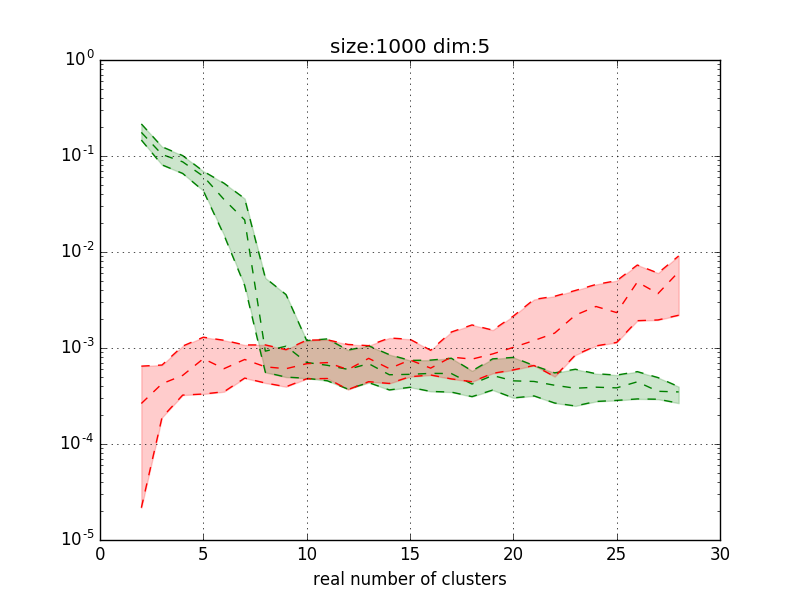
\includegraphics[width=300px]{./TeX_files/SparseWeightsVectorEstimation.png}
  \caption{Vert: Notre algorithme. Rouge: EM+BIC}
\end{figure}
%%!TEX root = ../main.tex

\chapter{Algorithm 2}

We consider the diagonal matrix $D_{\lambda}=diag(\lambda_1,\dots,\lambda_K)$.
\begin{figure}
\begin{center}
\mybox{
\begin{minipage}{0.85\linewidth}
\begin{algorithmic}%[1]\tt
%\SetLine%\SetAlgoLined
\small
\STATE {\bfseries Input:} data vectors $\bx_1,\ldots,\bx_n\in\RR^p$, the number of clusters $K$ and $D_{\lambda}$
\STATE {\bfseries Output:} parameter estimate $\hat\btheta = \{\hat\bmu_k,\hat\bOmega_k,\pi_k\}_{k\in[K]}$
\STATE {\tt 1: Initialize $t=0$, $\btheta=\btheta^0$.}
\STATE {\tt 2: {\bf Repeat}}
\STATE \qquad {\tt 3: Update the parameter $\bTau$:}
\begin{align*}
\tau_{i,k}^{t}  &= \frac{\pi_k^{t}\varphi_{\bmu_k^{t},\bOmega_k^{t}}(\bx_i)}{\sum_{k'\in[K]}\pi^{t}_{k'}\varphi_{\bmu^{t}_{k'},\bOmega^{t}_{k'}}(\bx_i)}.
\end{align*}
\STATE \qquad{\tt 4: Update the parameter $\btheta$:}
\begin{align*}
(\mu^k,B^k)&\in \argmin_{(\mu,B)\in \RR^p \times \RR^{p\times p},B_{jj}=1}\Big\{\frac{1}{N}\sum_{n=1}^N\tau_n^k(t)||(x_n-\mu)^TB||^2_2+||D_{\lambda}B||_{1,1}\Big\}\\
\pi_k^{t+1}     &= \\
\bmu_k^{t+1}    &= \\
\bOmega_k^{t+1} &
\end{align*}
\STATE \qquad {\tt 5: increment $t$: $t=t+1$}.
\STATE {\tt 6: {\bf Until} stopping rule.}
\STATE {\tt 7: {\bf Return} $\btheta^{t}$}.
\end{algorithmic}
\end{minipage}}
   \caption{Lasso for Gaussian mixtures}
   \label{algo:LassoGM}
\end{center}
\end{figure}

%!TEX root = ../main.tex

\section{structural analysis on $\bSigma$ approach}

We consider a multivariate Gaussian distribution with mean $\bmu^*$ and covariance $\bSigma^*$ and $Y_1,\dots,Y_N \in \RR^p$ iid drawn from this distribution. We would like to estimate $\bmu^*$ and $\bSigma^*$. We know that $\hat\bmu_n=\bar Y_n$, then wlog we consider $\mu^*=0$, the problem is to estimate $\bSigma^*$. We will study the precision matrix and consider that $\Sigma^{-1}$ is sparse. We note $\Sigma^{-1}=\Omega$, $Y_n$ the $n$-th random variable and $Y_n^i$ the $i$-th component of this vector.\
If $\Sigma^{-1}_{ij}=0 \Rightarrow Y^i \ci Y^j$ conditionally to $Y^{l\ne\{i,j\}}$. Thus, it makes sense to impose a $L_1$ penalty on $\Sigma^{-1}$ to increase its sparsity.

\subsection{Graphical Lasso}
Let consider a multivariate normal distribution with parameters $\mu^*,\; \Sigma^*$ with density;
\begin{equation}
\mathcal N(x|\mu^*,\Sigma^*)
=\frac{1}{(2\pi)^{d/2}|\Sigma^*|^{1/2}}\exp^{-\frac{1}{2}(x-\mu^*)^T\Sigma^{-1*}(x-\mu^*)}
\end{equation}
We consider $\mu=0$. Given N datapoints $X_1,\dots,X_N$ and $X_i \in \RR^d$, the log-likelihood is given by:
\begin{equation}
\begin{split}
\mathcal{L}(\Sigma)=\log\left(\prod_{n=1}^N\frac{1}{(2\pi)^{d/2}|\Sigma|^{1/2}}\exp^{-\frac{1}{2}(x_n)^T\Sigma^{-1}(x_n)}\right)\\
=-\frac{dN}{2}\log 2\pi - \frac{N}{2}\sum_{n=1}^N\log |\Sigma^*|- \frac{1}{2}\sum_{n=1}^N x_n^T\Sigma^{*,-1}x_n
\end{split}
\end{equation}
Note that $x_n^T\Sigma^{*,-1}x_n=tr(x_n^T\Sigma^{*,-1}x_n)$, and therefore:
\begin{equation}
\sum_{n=1}^N x_n^T\Sigma^{*,-1}x_n=tr\big(\sum_{n=1}^N x_n^T\Sigma^{*,-1}x_n\big)=tr\Big(\big[\sum_{n=1}^N x_n^Tx_n\big]\Sigma^{*,-1}\Big)=tr(S_N\Sigma^*)
\end{equation}
Where $S_N$ is the empirical covariance matrix. We can replace that in the log-likelihood expression:
\begin{equation}
\mathcal{L}(\Sigma)=-\frac{dN}{2}\log 2\pi - \frac{N}{2}\sum_{n=1}^N\log |\Sigma^*|- \frac{1}{2}tr(S_N\Sigma^*)
\end{equation}
Finally:
\begin{equation}
\mathcal{L}(\Sigma)=C+\frac{N}{2}\log|\Sigma^{-1}|-\frac{1}{2} tr(S_n\Sigma^{-1})
\end{equation}

Where C is a constant (dependent on N). Thus, considering the sparsity of the precision matrix $\Omega=\Sigma^{-1}$, we impose a penalization to the maximum likelihood estimator of $\Omega$
\begin{equation}
\hat\Omega\in argmin\big\{ \log|\Omega|-tr(S_N\Omega)-\lambda||\Omega||_1   \big\}
\end{equation}
A reason to use the $L_1$ penalization instead of the ridge is that for an $L_p$ penalization, the problem is convex for $p\geq 1$ and we have parsimonious property for $p\leq 1$.\
This is a convex optimization problem, however the complexity is $O(p^3)$ (Source, high dim \& var select Buhlmann 2006 ? Wassermann)

\subsection{Column-Wise Lasso}

We consider a gaussian vector $Y\in \RR^d$, $Y \sim \mathcal N(0,\Sigma)$. We can write $Y=(Y^1,Y^{2:d})$. With this decomposition we can write the covariance matrix as following:
\begin{equation}
\Sigma=
 \begin{pmatrix}
\sigma_1^2 & \Sigma_{12}\
\Sigma_{12}^T & \Sigma_{22}
\end{pmatrix}
\end{equation}
and according to theorem[?]: If $\Sigma_{22}$ is inversible, then:
\begin{equation}
\begin{array}{lcl}
\Ex[Y^1|Y^{2:d}]&=&\Sigma_{12}\Sigma_{22}^{-1}Y^{2:d}\\
Var[Y^1|Y^{2:d}]&=&\sigma_1^2-\Sigma_{12}\Sigma_{22}^{-1}\Sigma_{12}^T
\end{array}
\end{equation}
We have the following identity:
\begin{equation}
 \begin{pmatrix}
 \omega_{11}&\Omega_{12}\
 \Omega_{12}^T&\Omega_{22}
\end{pmatrix}
 \begin{pmatrix}
 \sigma_{1}^2&\Sigma_{12}\
 \Sigma_{12}^T&\Sigma_{22}
\end{pmatrix}
=
 \begin{pmatrix}
 1&0\
0&I_{p-1}
\end{pmatrix}
\end{equation}
Which gives the following equations:
\begin{equation}
  \begin{cases}
  \omega_{11}\sigma_1^2+\Omega_{12}\Sigma_{12}^T&=1\quad\,\quad(*) \\
  \omega_{11}\Sigma_{12}+\Omega_{12}\Sigma_{22}&=0\quad\,\quad(**)\\
  \Omega_{12}^T\Sigma_{12}+\Omega_{22}\Sigma_{22}&=I_{p-1}\quad(***)
  \end{cases}
\end{equation}
With (**) we have $-\omega_{11}\Sigma_{12}\Sigma_{22}^{-1}=\Omega_{12}$ and injected to (*) we have:
\begin{equation}
 \begin{cases}
 \Ex[Y^1|Y^{2:d}]&=-\frac{1}{\omega_{11}}\Omega_{12}Y^{2:d}\\
  Var[Y^1|Y^{2:d}]&=\frac{1}{\omega_{11}}
  \end{cases}
\end{equation}
Finally, $Y^1-\Ex[Y^1|Y^{2:d}]$ is a gaussian vector of $\RR^{d-1}$, centered, independent of $Y^{2:d}$ and of covariance matrix $\sigma_1^2-\Sigma_{12}\Sigma_{22}^{-1}\Sigma_{12}^T$. If we denote  $\xi^1\sim \mathcal N(0,1)$ we have $Y^1-\Ex[Y^1|Y^{2:d}]=\frac{1}{ \sqrt{\omega_{11}}}\xi^1$.\

Therefore, for $Y_1,\dots,Y_n$ iid of law $\mathcal N(0,\Sigma^*)$ we have:

\begin{equation}
\begin{array}{lcl}
  Y_i^1&=&-\frac{1}{\omega_{11}^*}\Omega_{12}Y_i^{2:d}+\frac{1}{\sqrt{\omega_{11}^*}}\xi^1_i\\
  &=&-\sum_{j=2}^{d}\frac{w_{ij}^*}{\omega_{11}^*}Y_i^j+\frac{1}{\sqrt{\omega_{11}^*}}\xi^1_i
\end{array}
\end{equation}

and
\begin{equation}
{\beta_1^*}^TY_i=\frac{1}{\sqrt{\omega_{11}^*}}\xi^1_i
\Rightarrow
{\beta_1^*}^T\bY=\frac{1}{\sqrt{\omega_{11}^*}}\bxi^1
\end{equation}
with
\begin{equation}
\beta_1^*=\frac{1}{\sqrt{\omega_{11}^*}}
  \begin{bmatrix}
  w_{11}^*\
  w_{12}\
  \vdots\
  w_{1d}
  \end{bmatrix}
  \in \RR^d
  \quad \text{and}\quad \bY= \begin{bmatrix}
  verifier\
  \end{bmatrix}
\end{equation}

\section{Overview}
